% Soubory musí být v kódování, které je nastaveno v příkazu \usepackage[...]{inputenc}

\documentclass[%        Základní nastavení
%  draft,    				  % Testovací překlad
  12pt,       				% Velikost základního písma je 12 bodů
  a4paper,    				% Formát papíru je A4
  oneside,      			% Jednostranný tisk
	%twoside,      			% Dvoustranný tisk (kapitoly a další důležité části tedy začínají na lichých stranách)
	unicode,						% Záložky a metainformace ve výsledném  PDF budou v kódování unicode
]{report}				    	% Dokument třídy 'zpráva', vhodná pro sazbu závěrečných prací s kapitolami

\usepackage[utf8]		  %	Kódování zdrojových souborů je UTF-8
	{inputenc}					% Balíček pro nastavení kódování zdrojových souborů

\usepackage[				% Nastavení geometrie stránky
	bindingoffset=10mm,		% Hřbet pro vazbu
	hmargin={25mm,25mm},	% Vnitřní a vnější okraj  (jsou nehezky shodné; jakási úroveň estetiky je dosažena pomocí hřbetu)
	vmargin={25mm,34mm},	% Horní a dolní okraj
	footskip=17mm,			  % Velikost zápatí
	nohead,					      % Bez záhlaví
	marginparsep=2mm,		  % Vzdálenost marginálií
	marginparwidth=18mm,	% Šířka marginálií
]{geometry}

\usepackage{sectsty}
	%přetypuje nadpisy všech úrovní na bezpatkové, kromě \chapter, která je přenastavena zvlášť v thesis.sty
	\allsectionsfont{\sffamily}

\usepackage{graphicx} % Balíček 'graphicx' pro vkládání obrázků
											% Nutné pro vložení logotypů školy a fakulty

\usepackage[          % Balíček 'acronym' pro sazby zkratek a symbolů
	nohyperlinks				% Nebudou tvořeny hypertextové odkazy do seznamu zkratek
]{acronym}						
											% Nutné pro použití prostředí 'acronym' balíčku 'thesis'

\usepackage[
	breaklinks=true,		% Hypertextové odkazy mohou obsahovat zalomení řádku
	hypertexnames=false % Názvy hypertext. odkazů budou tvořeny nezávisle na názvech TeXu
]{hyperref}						% Balíček 'hyperref' pro sazbu hypertextových odkazů
											% Nutné pro použití příkazu 'pdfsettings' balíčku 'thesis'

\usepackage{pdfpages} % Balíček umožňující vkládat stránky z PDF souborů
                      % Nutné při vkládání titulních listů a zadání přímo
                      % ve formátu PDF z informačního systému

\usepackage{enumitem} % Balíček pro nastavení mezerování v odrážkách
  \setlist{topsep=0pt,partopsep=0pt,noitemsep} % konkrétní nastavení

\usepackage{cmap} 		% Balíček cmap zajišťuje, že PDF vytvořené `pdflatexem' je
											% plně "prohledávatelné" a "kopírovatelné"

%\usepackage{upgreek}	% Balíček pro sazbu stojatých řeckých písmem
											%% např. stojaté pí: \uppi
											%% např. stojaté mí: \upmu (použitelné třeba v mikrometrech)
											%% pozor, grafická nekompatibilita s fonty typu Computer Modern!
                      
%\usepackage{amsmath} %balíček pro sabu náročnější matematiky                 

\usepackage{dirtree}	% sazba adresářové struktury
                      % vhodné pro prezentaci obsahu elektronické přílohy (např. CD)

\usepackage[formats]{listings}	% Balíček pro sazbu zdrojových textů
\lstset{              % nastavení
%	Definice jazyka použitého ve výpisech
%    language=[LaTeX]{TeX},	% LaTeX
%	language={Matlab},		% Matlab
	language={C},           % jazyk C
    basicstyle=\ttfamily,	% definice základního stylu písma
    tabsize=2,			% definice velikosti tabulátoru
    inputencoding=utf8,         % pro soubory uložené v kódování UTF-8
		columns=fixed,  %fixed nebo flexible,
		fontadjust=true %licovani sloupcu
    extendedchars=true,
    literate=%  definice symbolů s diakritikou
    {á}{{\'a}}1
    {č}{{\v{c}}}1
    {ď}{{\v{d}}}1
    {é}{{\'e}}1
    {ě}{{\v{e}}}1
    {í}{{\'i}}1
    {ň}{{\v{n}}}1
    {ó}{{\'o}}1
    {ř}{{\v{r}}}1
    {š}{{\v{s}}}1
    {ť}{{\v{t}}}1
    {ú}{{\'u}}1
    {ů}{{\r{u}}}1
    {ý}{{\'y}}1
    {ž}{{\v{z}}}1
    {Á}{{\'A}}1
    {Č}{{\v{C}}}1
    {Ď}{{\v{D}}}1
    {É}{{\'E}}1
    {Ě}{{\v{E}}}1
    {Í}{{\'I}}1
    {Ň}{{\v{N}}}1
    {Ó}{{\'O}}1
    {Ř}{{\v{R}}}1
    {Š}{{\v{S}}}1
    {Ť}{{\v{T}}}1
    {Ú}{{\'U}}1
    {Ů}{{\r{U}}}1
    {Ý}{{\'Y}}1
    {Ž}{{\v{Z}}}1
}

%%%%%vlastni balicky
\usepackage{makecell}
\usepackage{siunitx}
\sisetup{output-decimal-marker = {,}}
\DeclareSIUnit\LSB{LSB}
\sisetup{
  inter-unit-product=\ensuremath{{\cdot}},
%  tight-spacing=true,
}
\usepackage{subfigure}
\usepackage{tablefootnote}
\usepackage{amsmath}
\usepackage[thinc]{esdiff}



%%%%%%%%%%%%%%%%%%%%%%%%%%%%%%%%%%%%%%%%%%%%%%%%%%%%%%%%%%%%%%%%%
%%%%%%      Definice informací o dokumentu             %%%%%%%%%%
%%%%%%%%%%%%%%%%%%%%%%%%%%%%%%%%%%%%%%%%%%%%%%%%%%%%%%%%%%%%%%%%%

% V tomto souboru se nastavují téměř veškeré informace, proměnné mezi studenty:
% jméno, název práce, pohlaví atd.
% Tento soubor je SDÍLENÝ mezi textem práce a prezentací k obhajobě -- netřeba něco nastavovat na dvou místech.

\usepackage[
%%% Z následujících voleb jazyka lze použít pouze jednu
  czech-english,		% originální jazyk je čeština, překlad je anglicky (výchozí)
  %english-czech,	% originální jazyk je angličtina, překlad je česky
  %slovak-english,	% originální jazyk je slovenština, překlad je anglicky
  %english-slovak,	% originální jazyk je angličtina, překlad je slovensky
%
%%% Z následujících voleb typu práce lze použít pouze jednu
  semestral,		  % semestrální práce (výchozí)
  %bachelor,			%	bakalářská práce
  %master,			  % diplomová práce
  %treatise,			% pojednání o disertační práci
  %doctoral,			% disertační práce
%
%%% Z následujících voleb zarovnání objektů lze použít pouze jednu
%  left,				  % rovnice a popisky plovoucích objektů budou zarovnány vlevo
	center,			    % rovnice a popisky plovoucích objektů budou zarovnány na střed (vychozi)
%
]{thesis}   % Balíček pro sazbu studentských prací


%%% Jméno a příjmení autora ve tvaru
%  [tituly před jménem]{Křestní}{Příjmení}[tituly za jménem]
% Pokud osoba nemá titul před/za jménem, smažte celý řetězec '[...]'
\author{Marek}{Coufal}

%%% Identifikační číslo autora (VUT ID)
\butid{240598}

%%% Pohlaví autora/autorky
% (nepoužije se ve variantě english-czech ani english-slovak)
% Číselná hodnota: 1...žena, 0...muž
\gender{0}

%%% Jméno a příjmení vedoucího/školitele včetně titulů
%  [tituly před jménem]{Křestní}{Příjmení}[tituly za jménem]
% Pokud osoba nemá titul před/za jménem, smažte celý řetězec '[...]'
\advisor[Ing.]{Jan}{Král}[Ph.D.]

%%% Jméno a příjmení oponenta včetně titulů
%  [tituly před jménem]{Křestní}{Příjmení}[tituly za jménem]
% Pokud osoba nemá titul před/za jménem, smažte celý řetězec '[...]'
% Nastavení oponenta se uplatní pouze v prezentaci k obhajobě;
% v případě, že nechcete, aby se na titulním snímku prezentace zobrazoval oponent, pouze příkaz zakomentujte;
% u obhajoby semestrální práce se oponent nezobrazuje (jelikož neexistuje)
% U dizertační práce jsou typicky dva až tři oponenti. Pokud je chcete mít na titulním slajdu, prosím ručně odkomentujte a upravte jejich jména v definici "VUT title page" v souboru thesis.sty.
\opponent[doc.\ Mgr.]{Křestní}{Příjmení}[Ph.D.]

%%% Název práce
%  Parametr ve složených závorkách {} je název v originálním jazyce,
%  parametr v hranatých závorkách [] je překlad (podle toho jaký je originální jazyk).
%  V případě, že název Vaší práce je dlouhý a nevleze se celý do zápatí prezentace, použijte příkaz
%  \def\insertshorttitle{Zkác.\ náz.\ práce}
%  kde jako parametr vyplníte zkrácený název. Pokud nechcete zkracovat název, budete muset předefinovat,
%  jak se vytváří patička slidu. Viz odkaz: https://bit.ly/3EJTp5A
\title[Indoor Positioning Based on Inercial Measurement Unit
]{Měření polohy uvnitř budov pomocí inerciální jednotky
}

%%% Označení oboru studia
%  Parametr ve složených závorkách {} je název oboru v originálním jazyce,
%  parametr v hranatých závorkách [] je překlad
\specialization[Electronics and Communication Technologies]{Elektronika a komunikační technologie}

%%% Označení ústavu
%  Parametr ve složených závorkách {} je název ústavu v originálním jazyce,
%  parametr v hranatých závorkách [] je překlad
%\department[Department of Control and Instrumentation]{Ústav automatizace a měřicí techniky}
%\department[Department of Biomedical Engineering]{Ústav biomedicínského inženýrství}
%\department[Department of Electrical Power Engineering]{Ústav elektroenergetiky}
%\department[Department of Electrical and Electronic Technology]{Ústav elektrotechnologie}
%\department[Department of Physics]{Ústav fyziky}
%\department[Department of Foreign Languages]{Ústav jazyků}
%\department[Department of Mathematics]{Ústav matematiky}
%\department[Department of Microelectronics]{Ústav mikroelektroniky}
\department[Department of Radio Electronics]{Ústav radioelektroniky}
%\department[Department of Theoretical and Experimental Electrical Engineering]{Ústav teoretické a experimentální elektrotechniky}
%\department[Department of Telecommunications]{Ústav telekomunikací}
%\department[Department of Power Electrical and Electronic Engineering]{Ústav výkonové elektrotechniky a elektroniky}

%%% Označení fakulty
%  Parametr ve složených závorkách {} je název fakulty v originálním jazyce,
%  parametr v hranatých závorkách [] je překlad
%\faculty[Faculty of Architecture]{Fakulta architektury}
\faculty[Faculty of Electrical Engineering and~Communication]{Fakulta elektrotechniky a~komunikačních technologií}
%\faculty[Faculty of Chemistry]{Fakulta chemická}
%\faculty[Faculty of Information Technology]{Fakulta informačních technologií}
%\faculty[Faculty of Business and Management]{Fakulta podnikatelská}
%\faculty[Faculty of Civil Engineering]{Fakulta stavební}
%\faculty[Faculty of Mechanical Engineering]{Fakulta strojního inženýrství}
%\faculty[Faculty of Fine Arts]{Fakulta výtvarných umění}
%
%Nastavení logotypu (v hranatych zavorkach zkracene logo, ve slozenych plne):
\facultylogo[logo/FEKT_zkratka_barevne_PANTONE_CZ]{logo/VUT_barevne_PANTONE_CZ}

%%% Rok odevzdání práce
\graduateyear{2024}
%%% Akademický rok odevzdání práce
\academicyear{2023/24}

%%% Datum obhajoby (uplatní se pouze v prezentaci k obhajobě)
\date{5.\,1.\,2023} 

%%% Místo obhajoby
% Na titulních stránkách bude automaticky vysázeno VELKÝMI písmeny (pokud tyto stránky sází šablona)
\city{Brno}

%%% Abstrakt
\abstract[%
Překlad abstraktu
(v~angličtině, pokud je originálním jazykem čeština či slovenština; v~češtině či slovenštině, pokud je originálním jazykem angličtina)
]{%
Abstrakt práce v~originálním jazyce
}

%%% Klíčová slova
\keywrds[%
Překlad klíčových slov
(v~angličtině, pokud je originálním jazykem čeština či slovenština; v~češtině či slovenštině, pokud je originálním jazykem angličtina)
]{%
Klíčová slova v~originálním jazyce
}

%%% Poděkování
\acknowledgement{%
Rád bych poděkoval vedoucímu bakalářské/diplomové/disertační práce
panu Ing.~XXX YYY, Ph.D.\ za odborné vedení,
konzultace, trpělivost a~podnětné návrhy k~práci.
}%  % do tohoto souboru doplňte údaje o sobě, druhu práce, názvu...

%%%%%%%%%%%%%%%%%%%%%%%%%%%%%%%%%%%%%%%%%%%%%%%%%%%%%%%%%%%%%%%%%%%%%%%%

%%%%%%%%%%%%%%%%%%%%%%%%%%%%%%%%%%%%%%%%%%%%%%%%%%%%%%%%%%%%%%%%%%%%%%%%
%%%%%%     Nastavení polí ve Vlastnostech dokumentu PDF      %%%%%%%%%%%
%%%%%%%%%%%%%%%%%%%%%%%%%%%%%%%%%%%%%%%%%%%%%%%%%%%%%%%%%%%%%%%%%%%%%%%%
%% Při načteném balíčku 'hyperref' lze použít příkaz '\pdfsettings':
\pdfsettings
%  Nastavení polí je možné provést také ručně příkazem:
%\hypersetup{
%  pdftitle={Název studentské práce},    	% Pole 'Document Title'
%  pdfauthor={Autor studenstké práce},   	% Pole 'Author'
%  pdfsubject={Typ práce}, 						  	% Pole 'Subject'
%  pdfkeywords={Klíčová slova}           	% Pole 'Keywords'
%}
%%%%%%%%%%%%%%%%%%%%%%%%%%%%%%%%%%%%%%%%%%%%%%%%%%%%%%%%%%%%%%%%%%%%%%%

\pdfmapfile{=vafle.map}

%%%%%%%%%%%%%%%%%%%%%%%%%%%%%%%%%%%%%%%%%%%%%%%%%%%%%%%%%%%%%%%%%%%%%%%
%%%%%%%%%%%       Začátek dokumentu               %%%%%%%%%%%%%%%%%%%%%
%%%%%%%%%%%%%%%%%%%%%%%%%%%%%%%%%%%%%%%%%%%%%%%%%%%%%%%%%%%%%%%%%%%%%%%
\begin{document}
\pagestyle{empty} %vypnutí číslování stránek

%%% Vložení desek -- od září 2021 na žádost fakulty nepoužíváno
%\includepdf[pages=1]%  buďto generovaných informačním systémem
  %{pdf/student-desky}% název souboru nesmí obsahovat mezery!
%%% NEBO vytvoření desek z balíčku
%%\makecover
%%%
%\oddpage % při dvojstranném tisku přidá prázdnou stránku
%% kazdopádně ale:
%\setcounter{page}{1} %resetovaní čítače stránek -- desky do číslování nezahrnujeme

%% Vložení titulního listu
\includepdf[pages=1]%    buďto generovaného informačním systémem
  {pdf/student-titulka}% název souboru nesmí obsahovat mezery!
%% NEBO vytvoření titulní stránky z balíčku
%\maketitle
%%
\oddpage  % při dvojstranném tisku se přidá prázdná stránka
   
%% Vložení zadání
\includepdf[pages=1]%   buďto generovaného informačním systémem
  {pdf/student-zadani}% název souboru nesmí obsahovat mezery!
%% NEBO lze vytvořit prázdný list příkazem ze šablony
%\patternpage{}%
%	{\sffamily\Huge\centering ZDE VLOŽIT LIST ZADÁNÍ}%
%	{\sffamily\centering Z~důvodu správného číslování stránek}
%%
\oddpage% při dvojstranném tisku se přidá prázdná stránka

%% Vysázení stránky s abstraktem
\makeabstract

% Vysázení stránky s rozšířeným abstraktem
% (pokud píšete práci v češtině či slovenštině, vložení rozšířeného abstraktu zrušte;
%  pro semestrální projekt také není potřeba rozšířený abstrakt uvádět)
%% Vysázení stránky s rozšířeným abstraktem
% (týká se pouze bc. a dp. prací psaných v angličtině, viz Směrnice rektora 72/2017)
\cleardoublepage
\noindent
{\large\sffamily\bfseries\MakeUppercase{Rozšířený abstrakt}}
\\
Výtah ze směrnice rektora 72/2017:\\
\emph{Bakalářská a diplomová práce předložená v angličtině musí obsahovat rozšířený abstrakt v češtině
nebo slovenštině (čl. 15). To se netýká studentů, kteří studují studijní program akreditovaný v
angličtině.}
(čl. 3, par. 7)\\
\emph{Nebude-li vnitřní normou stanoveno jinak, doporučuje se rozšířený abstrakt o rozsahu přibližně 3
normostrany, který bude obsahovat úvod, popis řešení a shrnutí a zhodnocení výsledků.}
(čl. 15, par. 5)

%%% Vysázení citace práce
\makecitation

%%% Vysázení prohlášení o samostatnosti
\makedeclaration

%%% Vysázení poděkování
\makeacknowledgement

%%% Vysázení obsahu
\tableofcontents

%%% Vysázení seznamu obrázků
% (vynechejte, pokud máte dva nebo méně obrázků)
\listoffigures

%%% Vysázení seznamu tabulek
% (vynechejte, pokud máte dvě nebo méně tabulek)
\listoftables

%%% Vysázení seznamu výpisů kódu
% (vynechejte, pokud máte dva nebo méně výpisů)
%\lstlistoflistings

\cleardoublepage\pagestyle{plain}   % zapnutí číslování stránek

%Pro vkládání kapitol i příloh používejte raději \include než \input
%%% Vložení souboru 'text/uvod.tex' s úvodem
\chapter*{Úvod}
\phantomsection
\addcontentsline{toc}{chapter}{Úvod}

Tato práce se zabývá poměrně komplexní problematikou inerciální navigace pro použití uvnitř budov a jejím sestrojením, tedy určováním polohy pomocí „black boxu“ který své údaje o pohybu určí primárně z údajů o lineárním zrychlení z akcelerometru a úhlové rychlosti z gyroskopu pro omezení potřeby neustálé dostupnosti signálu z globálních navigačních systémů.

Jsou popsány algoritmy pro zpracování dat šestiosé inerciální jednotky s nehybně umístěnými \ac{MEMS} gyroskopy a akcelerometry, což umožňuje značnou miniaturizaci a snížení ceny, v porovnání s osvědčenými systémy využívající velké a složité mechanické konstrukce gimbalů a gyroskopů. Přestože se přesnost senzorů stále zlepšuje, i díky malé odchylce měřených dat může rychle narůstat chyba odhadované polohy díky integraci úhlové rychlosti a dvojité integraci lineárního zrychlení. Z tohoto důvodu je jednotka opatřena i magnetometrem a \ac{GNSS} modulem pro možnost fúze dalších dat pro co největší zmenšení chyby, tomuto se ovšem bude věnovat až navazující bakalářská práce.

Jsou také věnovány kapitoly samotnému návrhu inerciální jednotky, minimálním požadavkům na komunikace a jejich počtům a rychlostem, způsobu zaznamenávání dat a celkovému blokovému konceptu. V poslední kapitole je také popsán návrh desky plošných spojů inerciální jednotky. 

%%% Vložení souboru 'text/cile.tex' s úvodem
%\chapter*{Cíle práce}
\phantomsection
\addcontentsline{toc}{chapter}{Cíle práce}

Konkrétní specifikace cílů, které má autor v~práci vyřešit.
Tato kapitola je \emph{volitelná} -- pokud váš studijní program nevyžaduje zvláštní kapitolu s cíli,
cíle specifikujte v~rámci Úvodu.

\chapter{Algoritmus inerciální navigace} \label{INSalg}
\section{Využití inerciální navigace}
Možnost navigace a znalost polohy je pro lidstvo již dlouhou dobu důležitá jak v průmyslu, tak i v každodenním životě. Pravděpodobně nejrozšířenějším druhem navigace jsou tzv. globální navigační systémy, například globální polohový systém (\emph{Global Positioning System}, \acsu{GPS}). Ovšem pro některé aplikace nemusí být použití \ac{GNSS}, ať už z politických či technických důvodů ideální. Pro navigaci v oblasti letectví a námořnictví se začala inerciální navigace využívat kolem roku 1960 a je využívána dodnes. \cite{Tittertonc2004}

Díky stále přesnějším a levnějším inerciálním senzorům se rozšiřují možnosti využití inerciální navigace i v běžných průmyslových aplikacích, například v oblastech robotiky, automobilové techniky, nebo i pro údržbu podzemních infrastruktur, mapování kanalizací a další. \cite{Tittertonc2004} Tato práce se zabývá využitím inerciální navigace pro účely určení polohy uvnitř budov a fúzí dat z dalších senzorů.

\section{Princip fungování inerciální navigace} \label{INSPrinciple}
Inerciální navigační systémy pracují na principu nepřímého měření z dat, které poskytuje akcelerometr a gyroskop.   
Akcelerometry poskytují informaci o lineárním zrychlení v prostoru pomocí měření síly $ F $ na definovanou jednotku hmotnosti $ m $ a pomocí druhého Newtonova zákona určí zrychlení $ a $ \cite{Tittertonc2004}

\begin{equation} \label{eq:2NZ}
a=\frac{F}{m} .
\end{equation}

Síla $ F $ představuje síly působící na senzor vůči jeho tělu ve volném pádu, skládá se tedy ze statické (tíhové) a dynamické síly způsobené zrychlením vůči Zemi. \cite{Tittertonc2004}
Z tohoto důvodu, pokud je akcelerometr v klidu na povrchu Země, změří zrychlení o velikosti zhruba \SI{9,81}{\meter\per\second\squared}.

Akcelerometry zpravidla měří hodnoty lineárního zrychlení ve třech navzájem pravoúhlých osách. Znalostí počáteční rychlosti $ v(t_{0}) $ a polohy $ x(t_{0}) $ v čase $ t_{0} $ můžeme pomocí zrychlení $ a $ v časech $ s>t_{0} $ určit rychlost $ v(t) $ a následně polohu $ x(t) $ pomocí dvou integrací \cite{Grewal2013}

\begin{equation}
v(t)=v(t_{0}) + \int_{t_{0}}^{t} a(s) \dif s ,
\end{equation}
\begin{equation}
x(t)=x(t_{0}) + \int_{t_{0}}^{t} v(s) \dif s .
\end{equation}

Aby bylo možné s inerciální jednotkou volně pohybovat v prostoru, je potřeba kromě znalosti polohy měřit, nebo kompenzovat její natočení. 
Jednou z možností jak kompenzovat rotaci jednotky je připevněním akcelerometrů na gimbal, který bude udržovat jejich natočení vůči Zemi konstantní. Tohoto principu se často využívá v letectví, zejména kvůli jejich vysoké přesnosti, ovšem velkou nevýhodou bývá mechanická složitost a velikost. \cite{Grewal2013} \cite{Polak2018}

Druhou možností, jak kompenzovat natočení je měřit jeho úhel a následně zrychlení z akcelerometru rotovat vůči referenčnímu systému.\cite{Grewal2013} \cite{Polak2018}
K tomuto účelu slouží gyroskopy, které měří úhlovou rychlost $ \omega $ otáčení jednotky kolem osy. Podobně jako se zrychlením u akcelerometru, znalostí počátečního úhlu $ \varphi (t_{0}) $ v čase $ t_{0} $ můžeme pomocí úhlové rychlosti $ \omega $ v časech $ s>t_{0} $ určit úhel natočení $ \varphi (t) $, ovšem tentokrát pouze jednou integrací

\begin{equation}
\varphi (t)=\varphi (t_{0}) + \int_{t_{0}}^{t} \omega (s) \dif s .
\end{equation}

Díky tomu můžou být gyroskopy a akcelerometry nepohyblivě připevněny na mechanickou konstrukci. Jde o tzv. „Strapdown“ typ inerciální navigace.

\subsection{Zavedení vztažných soustav}
Pro účely přehlednosti a exaktnosti bývá v oblastech inerciální navigace zavedeno několik kartézských vztažných soustav. Každá soustava je ortogonální a pravotočivá. \cite{Pekarek2020} \cite{Tittertonc2004} 

\begin{itemize}
\item Inertial frame (i-frame) má počátek ve středu Země. Její osy jsou pevné vůči nepohybujícím se hvězdám. Osa $ z_{i} $ prochází zemskou osou.
\item Earth frame (e-frame) má také počátek ve středu Země, její osy jsou pevně vztažené vůči Zemi, tedy rotují kolem i-frame. Osa $ z_{e} $ prochází zemskou osou.
\item Navigation frame (n-frame) má počátek ve výchozím bodě navigace. Osy jsou natočené ve směrech sever, východ, dolů (\emph{North East Down}, \acsu{NED}).
\item Body frame (b-frame) má počátek v inerciální jednotce a její osy jsou natočené ve směrech náklonu, stáčení a vychýlení jednotky.
\end{itemize}

S následnými měřenými a vypočtenými daty je často manipulováno jako s vektory označenými indexy odpovídajícím soustavě, ke které jsou vztaženy (i,~e,~n,~b).

\section{Vztažné soustavy a rotace Země}
Pokud budeme chtít provozovat navigaci vztaženou k pevnému počátečnímu bodu v prostoru (i-frame), bude možné používat klasické pohybové rovnice, tedy pro zrychlení $ \vec{a}_{i} $, polohu $ \vec{r} $ a čas $ t $ platí \cite{Tittertonc2004} 

\begin{equation} \label{eq:aiDiff}
\vec{a}_{i} = \left. \diff[2]{\vec{r}}{t} \right|_{i}
\end{equation}

a obdobně pro rychlost $ \vec{v}_{i} $ platí

\begin{equation}
\vec{v}_{i} = \left. \diff{\vec{r}}{t} \right|_{i} .
\end{equation}

Ovšem v mnoha případech použití inerciální navigace potřebujeme jako počátek zvolit nějaký bod na Zemi, která se neustále otáčí kolem své osy, v tomto případě tedy budeme využívat e-frame. Pokud máme data pouze ze vztažné soustavy i-frame, bude potřeba započíst úhlovou rychlost Země $ \vec{\omega_{ie}} $ \cite{Tittertonc2004} 

\begin{equation}
\vec{\omega_{ie}} = \begin{pmatrix} 0 \\ 0 \\ \Omega \end{pmatrix} ,
\end{equation}

kde $ \Omega = \SI{7,292E-5}{\radian\per\second}$ je rychlost rotace Země kolem své osy, vztaženo vůči nejbližší hvězdě (Slunci). Poté můžeme rychlost $ \vec{v}_{e} $ v e-framu definovat jako \cite{Tittertonc2004} \cite{Grewal2013}

\begin{equation}
\vec{v}_{e} = \left. \diff{\vec{r}}{t} \right|_{e} = \vec{v}_{i} - \vec{\omega_{ie}} \times \vec{r} .
\end{equation}

S přepočty mezi i a e frame je potřeba nakládat zejména při navigaci letadel a raket, kdy je potřeba započíst i rotaci Země, vzhledem k dlouhým úsekům času i vzdálenosti. V této práci se ovšem zabýváme navigací na malé vzdálenosti, kdy doba měření může být řádově v jednotkách minut a vzdálenost ve stovkách metrů. Vliv rotace Země tedy bude velmi malý.

\section{Tíhové pole Země}
Abychom mohli popsat chování jednotky v i-frame, označíme dynamickou sílu způsobenou zrychlením na jednotku hmotnosti jako tzv. „specifickou sílu“ $ \vec{f} $ představující sílu na jednotku hmotnosti, tedy samotné zrychlení. S její pomocí můžeme rovnici \ref{eq:aiDiff} upravit na \cite{Tittertonc2004} \cite{Grewal2013}

\begin{equation} \label{eq:aiDiffFG}
\vec{a}_{i} = \left. \diff[2]{\vec{r}}{t} \right|_{i} = \vec{f} + \vec{g} ,
\end{equation}

kde $ \vec{g} $ je tíhové zrychlení pole Země.
Z tohoto poznatku vyplývá, že pro správné fungování inerciální navigace je potřeba přesně znát velikost a směr $ \vec{g} $. 

Vzhledem k tomu, že Země: \cite{Halliday2000}
\begin{itemize}
\item rotuje kolem své osy,
\item není koule,
\item není homogení,
\end{itemize}
není možné považovat velikost tíhového zrychlení za konstantní a jeho směr vždy do středu Země.

Rotace Země kolem své osy vyvolává dostředivé zrychlení.\footnote{Všude na Zemi, vyjma samotných zeměpisných pólů}
Toto zrychlení má vždy kolmý směr k ose otáčení Země. Vektorovým součtem s gravitačním zrychlením $ \vec{a_{g}} $, které má vždy směr do středu Země dostaneme tíhové zrychlení $ \vec{g} $, proto se v závislosti na zeměpisné šířce tíhové zrychlení odchyluje od středu Země. \cite{Halliday2000}

Pro kompenzaci rotace Země bychom mohli vyjádřit tíhové zrychlení $ \vec{g} $ v závislosti na gravitačním zrychlení $ \vec{a_{g}} $ a následně využít v rovnici \ref{eq:aiDiffFG} \cite{Tittertonc2004}

\begin{equation} \label{eq:coriolis}
\vec{g}=\vec{a_{g}} - \vec{\omega_{ie}} \times (\vec{\omega_{ie}} \times \vec{r}) .
\end{equation}

Díky tomu, že Země není koule, ale přibližně elipsoid, jsou body na pólech blíž středu Země než body na rovníku, to tedy ovlivňuje velikost gravitačního zrychlení. Tento vliv by šel analyticky vypočítat, pokud bychom předpokládali, že Země je elipsoid a zanedbali vliv reliéfu povrchu Země. \cite{Halliday2000}

Vzhledem k tomu, že tato práce se zabývá zpracováním dat z inerciální navigace až tzv. offline, tedy ne v reálném čase, můžeme pro řešení problémů s nekonzistentním tíhovým polem Země použít některý z dostupných gravitačních modelů Země (\emph{Earth
Gravitational Model}, \acsu{EGM}).

\subsection{Gravitační modely Země}
\ac{EGM} jsou modely popisující geoid Země s velmi širokou škálou použití v oblastech fyziky, geodézie, oceánografie, navigace a dalších. Spravuje je americká geoprostorová agentura (\emph{National Geospatial-
Intelligence Agency}, \acsu{NGA}) a jsou volně dostupné. Nejnovější věřejně dostupný \ac{EGM} je z roku 2008 (EGM2008), který byl vytvořen na základě několika pozemních a výškových měření. \cite{Pavlis2012}

Vytvořená mapa s výškou geoidu modelu EGM2008 publikovaného \ac{NGA} je znázorněna na obrázku \ref{fig:EGM2008}

\begin{figure}[h] 
    \centering
    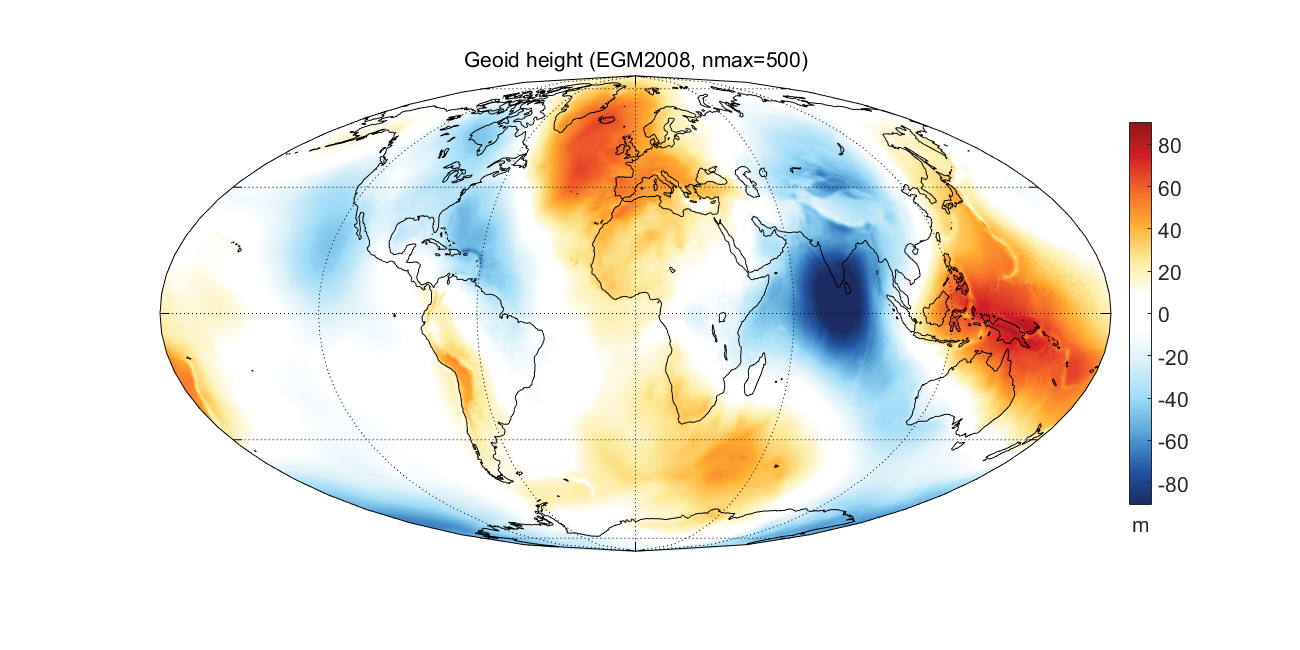
\includegraphics[width=0.8\textwidth]{obrazky/EGM2008}
    \caption{Výškový reliéf geoidu. \cite{Bezdek2013}}
    \label{fig:EGM2008}
\end{figure}

Takovýto model je poté možné použít například pomocí funkcí z Matlab Aerospace Toolbox, který vypočítá vektor gravitačního zrychlení $ a_{g} $ se správným směrem i velikostí na základě dodaný souřadnic systému WGS84. Poté pomocí rovnice \ref{eq:coriolis} můžeme vypočítat tíhové zrychlení.

\section{Rotace měření akcelerometru}
Vzhledem k tomu, že se tato práce zabývá strapdown systémem inerciální navigace, jsou data akcelerometru vztažena k soustavě inerciální jednotky (tedy b-frame). Pro převedení dat do vztažné soustavy i-frame je potřeba rotovat vektor specifické síly $ \vec{f} $ maticí směrových kosínů $ \mathbf{C}_{b}^{i} $. Tato rotace by se dala popsat jako 3 po sobě jdoucí natočení o tzv. Eulerovy úhly vůči referenčním osám (např. pro tento případ i-frame). Tyto úhly označíme $ \phi $, $ \theta $ a $ \psi $. \cite{Tittertonc2004}

\begin{itemize}
\item Rotaci o úhel $ \phi $ kolem osy x přiřadíme rotační matici $ \mathbf{C}_{x} $ \cite{Tittertonc2004}
\begin{equation}
\mathbf{C}_x=\left[\begin{array}{ccc}
1 & 0 & 0 \\
0 & \cos \phi & -\sin \phi \\
0 & \sin \phi & \cos \phi
\end{array}\right] .
\end{equation}

\item Rotaci o úhel $ \theta $ kolem osy y přiřadíme rotační matici $ \mathbf{C}_{y} $ \cite{Tittertonc2004}
\begin{equation}
\mathbf{C}_y=\left[\begin{array}{ccc}
\cos \theta & 0 & \sin \theta \\
0 & 1 & 0 \\
-\sin \theta & 0 & \cos \theta
\end{array}\right] .
\end{equation}

\item Rotaci o úhel $ \psi $ kolem osy z přiřadíme rotační matici $ \mathbf{C}_{z} $ \cite{Tittertonc2004}
\begin{equation}
\mathbf{C}_z=\left[\begin{array}{ccc}
\cos \psi & -\sin \psi & 0 \\
\sin \psi & \cos \psi & 0 \\
0 & 0 & 1
\end{array}\right] .
\end{equation} 

\end{itemize}

Součinem těchto tří matic získáme matici směrových kosinů $ \mathbf{C_{b}^{i}} $ pro převod z b-frame na i-frame \cite{Tittertonc2004}
\begin{equation}
\mathbf{C}_{b}^{i}= (\mathbf{C}_{i}^{b})^{\mathrm{T}} = (\mathbf{C}_{x}\mathbf{C}_{y}\mathbf{C}_{z})^{\mathrm{T}} = \mathbf{C}_{z}^{\mathrm{T}}\mathbf{C}_{y}^{\mathrm{T}}\mathbf{C}_{x}^{\mathrm{T}} ,
\end{equation}

\begin{equation}
\mathbf{C}_{b}^{i}=
\left[\begin{array}{ccc}
\cos \theta \cos \psi & -\cos \phi \sin \psi+\sin \phi \sin \theta \cos \psi & \sin \phi \sin \psi+\cos \phi \sin \theta \cos \psi \\
\cos \theta \sin \psi & \cos \phi \cos \psi+\sin \phi \sin \theta \sin \psi & -\sin \phi \cos \psi+\cos \phi \sin \theta \sin \psi \\
-\sin \theta & \sin \phi \cos \theta & \cos \phi \cos \theta
\end{array}\right] .
\end{equation}

Toto poté můžeme použít k rotaci samotného vektoru specifické síly $ \vec{f} $ z b-frame na i-frame

\begin{equation}
\vec{f^{i}} = \mathbf{C}_{b}^{i}\vec{f^{b}} .
\end{equation}

Kombinací s rovnicí \ref{eq:aiDiffFG} získáme rovnici popisující pohyb

\begin{equation}
\vec{a}_{i} = \left. \diff[2]{\vec{r}}{t} \right|_{i} = \vec{f^{i}} + \vec{g^{i}} = \mathbf{C}_{b}^{i}\vec{f^{b}} + \vec{g^{i}} .
\end{equation}
\section{Diagram algoritmu inerciální navigace}
Pro přehlednější znázornění algoritmu základní formy inerciální navigace pro 6 stupňů volnosti (\emph{Degrees
of Freedom}, \acsu{DoF}) inerciální měřicí jednotky (\emph{Inertial Measurement Unit}, \acsu{IMU}) byl vytvořen blokový diagram (obrázek \ref{StrapdownBlock}).

\begin{figure}[h]
    \centering
    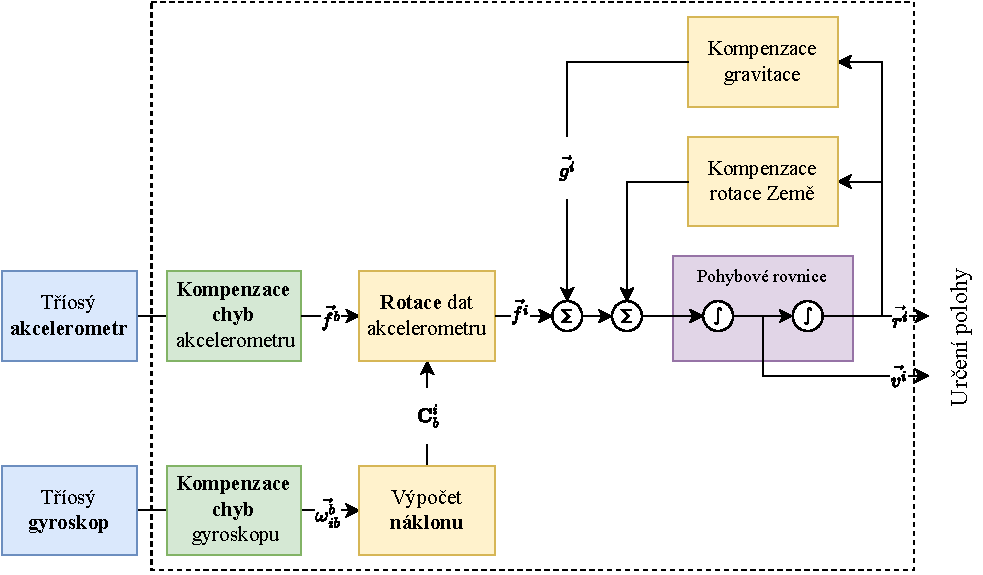
\includegraphics[width=\textwidth]{obrazky/StrapdownBlock}
    \caption{Blokové schéma algoritmu strapdown inerciální navigace, převzato z \cite{Tittertonc2004} \cite{Grewal2013}. }
    \label{StrapdownBlock}
\end{figure}

\chapter{Inerciální senzory}
Ke sběru dat pro účely inerciální navigace se jako první začaly používat a stále používají např. v letectví složité, velké a drahé mechanické přístroje se setrvačníky poháněnými motory využívající gyroskopický efekt. Jejich natočení os vůči referenčnímu rámu je poté možné měřit například laserem, či jiným způsobem. Tyto senzory jsou díky jejich přesnosti stále využívány v aplikacích, kde je kladen důraz na opravdu velkou spolehlivost a přesnost. Ovšem díky zlepšujícím se technologiím se začínají hojně využívat i \ac{MEMS} \ac{IMU} v oblastech inerciální navigace, zejména tam, kde nejsou kladeny velmi přísné požadavky na přesnost a spolehlivost, jako je například navigace uvnitř budov. Díky \ac{MEMS} technologiím je možné sestrojit celou inerciální jednotku bez jakýchkoliv pohyblivých částí, velmi malou a poměrně levnou. \cite{Tittertonc2004} \cite{Grewal2013}

\section{MEMS akcelerometry} \label{MEMSaccel}
Akcelerometr měří lineární zrychlení nepřímo díky 2. Newtonovu zákonu (rovnice \ref{eq:2NZ}). Přímo na struktuře křemíku je těleso známé hmotnosti, kterému je umožněn pružný pohyb v nějaké z os. Pokud na akcelerometr působí zrychlení, je těleso vychylováno silou, která je následně měřena. Tato síla je často měřena jako změna kapacity mechanické struktury znázorněné na obrázku \ref{fig:MEMSaccelerometer} a \ref{fig:MEMSaccelerometerPhoto}, převedena na napětí, zesílena, vyfiltrována a následně převedena \ac{ADC} převodníkem.
Tyto struktury jsou následně uspořádány ortogonálně, aby vytvořily tříosý akcelerometr. \cite{Dadafshar2014}

\begin{figure}[h]
    \centering
    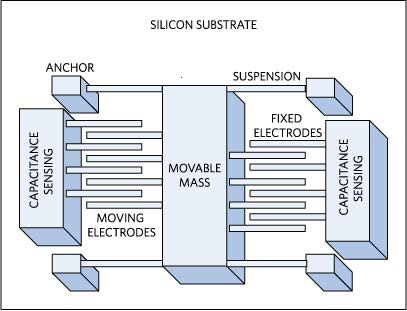
\includegraphics[width=0.5\textwidth]{obrazky/MEMSaccelerometer}
    \caption{Struktura MEMS akcelerometru. \cite{Dadafshar2014}}
    \label{fig:MEMSaccelerometer}
\end{figure}

Za povšimnutí stojí rozdílné parametry např. biasu pro různé osy \ac{IMU} v tabulce \ref{table:fyzikalniPorovnaniIMU}, to může být způsobené vrstvením struktury během výroby čipu, kdy dvě z os akcelerometru mají osy vychýlení hmoty rovnoběžnou se směry vrstev, zatímco třetí osa je na tyto vrstvy kolmá.

\begin{figure}[h]
    \centering
    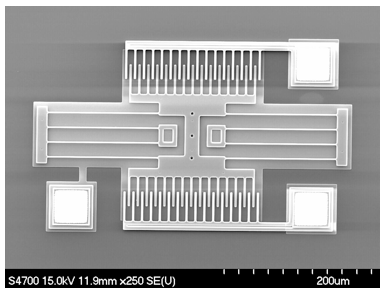
\includegraphics[width=0.5\textwidth]{obrazky/MEMSaccelerometerPhoto}
    \caption{Mikroskopický snímek MEMS akcelerometru. \cite{cCumN04KaPNjERaF}}
    \label{fig:MEMSaccelerometerPhoto}
\end{figure}

\section{MEMS gyroskopy}
Gyroskopy jsou senzory, které měří úhlovou rychlost. Uspořádání mechanické struktury (na obrázku \ref{fig:MEMSgyroscope}) je rozdílné v porovnání s akcelerometry. Zde je tělesu definované hmotnosti umožněno kmitat v jedné z os. Při působení úhlové rychlosti na gyroskop je vnitřní struktura díky Coriolisově síle vychýlena, což způsobí změnu kapacity. Ta je dále zpracována obdobně jako v akcelerometru (kapitola \ref{MEMSaccel}). \cite{Tittertonc2004} \cite{Dadafshar2014}
\begin{figure}[h]
    \centering
    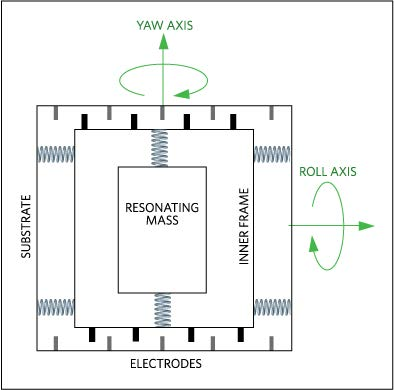
\includegraphics[width=0.5\textwidth]{obrazky/MEMSgyroscope}
    \caption{Struktura MEMS gyroskopu. \cite{Dadafshar2014}}
    \label{fig:MEMSgyroscope}
\end{figure}

\chapter{Hardware inerciální jednotky}

\begin{figure}[h]
    \centering
    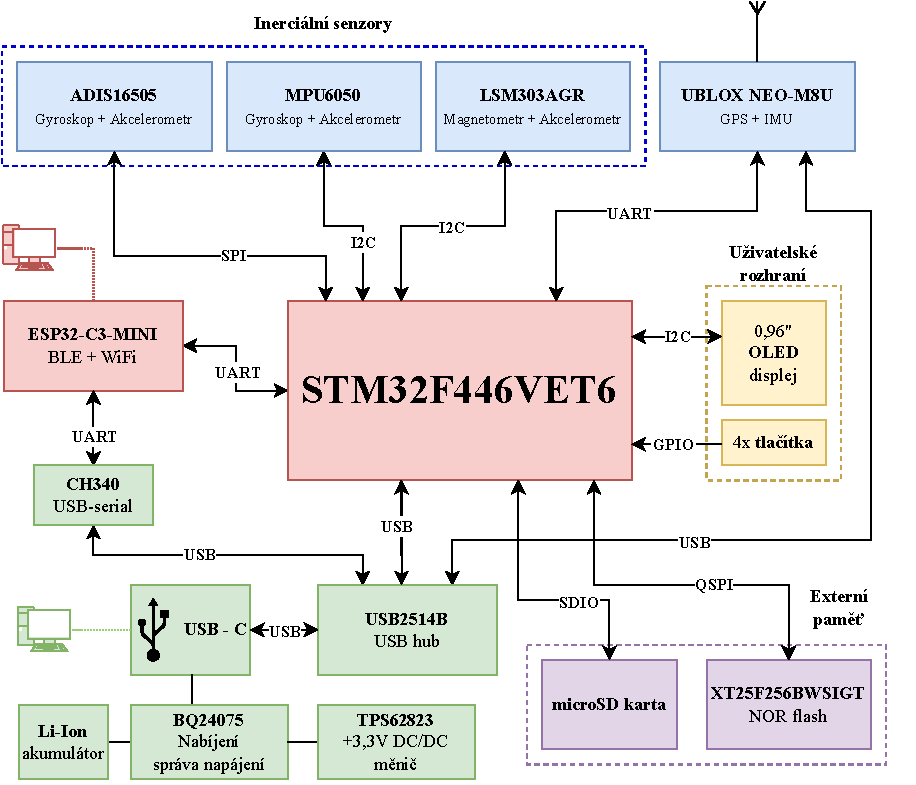
\includegraphics[width=\textwidth]{obrazky/IMUnav_H00_block}
    \caption{Blokové schéma inerciální jednotky.}
\end{figure}

Hardware inerciální jednotky je realizován tak, aby umožňoval zaznamenávat hodnoty změřené inerciálními senzory a poskytovat dohromady devítiosé data (akcelerometr, gyroskop a magnetometr). Jednotka také obsahuje \ac{GPS} modul s vestavěným \ac{IMU}, jehož použití by mohlo být vhodné například v prostorech s alespoň částečným pokrytím signálu \ac{GPS}.

Naměřená data je možné uložit do externí NOR Flash paměti připojené k mikrokontroléru (\emph{Microcontroller
Unit}, \acsu{MCU}), popřípadě lze využít i kartu typu microSD. Konektor univerzální sériové sběrnice (\emph{Universal Serial Bus}, \acsu{USB}) typu C umožňuje nabíjení vestavěného Li-Ion akumulátoru jednotky a komunikaci mezi PC a ESP32, \ac{GPS} modulem a hlavním \ac{MCU} skrze vestavěný \ac{USB} rozbočovač. K přenosu dat pro jejich následné zpracování v PC primárně slouží USB rozhraní, ale zařízení disponuje i bezdrátovým modulem ESP32-C3, umožňující komunikaci přes WiFi, nebo Bluetooth.

Pro jednoduchou volnost pohybu je jednotka napájena jedním Li-Ion akumulátorem velikosti 18650, při záznamu dat tedy nebude potřeba externího zdroje energie. Grafický organický LED (\emph{Organic Light-Emitting Diode}, \acsu{OLED}) displej a 4 tlačítka slouží jako uživatelské rozhraní při používání jednotky.

\section{Akcelerometr a gyroskop} \label{AccGyroText}
Jednotka obsahuje dvě šestiosá \ac{IMU} (gyroskop s akcelerometrem) rozdílných parametrů a řádově rozdílné ceny. Takto odlišné součástky byly vybrány proto, aby bylo možné porovnat vliv přesnosti, šumu, biasu a driftu senzorů na následně zpracovaná data.
V tabulce \ref{table:fyzikalniPorovnaniIMU} jsou porovnány důležité parametry senzorů MPU6050 a ADIS16505-2. Pro účely inerciální navigace je důležitý zejména nízký bias a drift senzorů, aby při integraci dat k vyhodnocení polohy nebyla integrována i driftová chyba, což má za výsledek velmi nepřesné zpracování hodnot. \cite{Blocher2021322}

Integrovaný obvod MPU6050 je standardní šestiosé \ac{MEMS} \ac{IMU}, vhodné mimo jiné pro použití v mobilních zařízeních a dalších podobných aplikacích. Jeho vnitřní gyroskop a akcelerometr má softwarově přepínatelné rozsahy měřených veličin. Kromě inerciálních senzorů má i vestavěný signálový procesor pro fúzi a filtrování dat přímo v integrovaném obvodu. Tato funkce může být vhodná pro odlehčení výpočetního výkonu hlavního procesoru, ovšem pro účely této práce nebude signálový procesor využit, jelikož se měřená data budou zpracovávat až po jejich naměření v PC, ne v reálném čase. Vzorkovací frekvence gyroskopu je 8 kHz a akcelerometru 1 kHz, oba senzory mají 16bitové rozlišení.
\cite{euxR3Yh5ol4JWNAi}

MPU6050 disponuje rozhraním mezi-obvodové komunikace (\emph{Inter-Integrated Circuit}, \acsu{I2C}) s maximální frekvencí hodinového signálu 400 kHz. \cite{euxR3Yh5ol4JWNAi}
Pokud bychom chtěli vyčítat ze senzoru data při maximální možné vzorkovací frekvenci, byla by potřeba minimální přenosová rychlost sběrnice
\begin{equation}
f_{\
mathrm{clk}}=3~\mathrm{osy} \cdot(f_{\mathrm{gyro}} + f_{\mathrm{acc}})\cdot (\mathrm{16bitů} + 2 \cdot \mathrm{ACK})=3\cdot(8000+1000)\cdot(16+2)=\SI{486}{\kilo\hertz} .
\end{equation}
Při vyčítání dat o maximální vzorkovací frekvenci jsme omezeni samotným \ac{I2C} rozhraním senzoru (využití maximální vzorkovací frekvence je teoreticky možné krátkodobě, pomocí interního 1kB FIFO zásobníku).\cite{euxR3Yh5ol4JWNAi}

Jelikož pro účely inerciální navigace stačí vzorkovací frekvence dat v  řádu stovek hertz \cite{Wei2022}, tak není tato limitace omezující. Senzor je propojen s hlavním \ac{MCU} přes \ac{I2C} sběrnici s frekvencí hodinového signálu 400 kHz a není sdílena s žádným jiným zařízením, aby bylo možné, v případě potřeby, využít maximální dostupný potenciál senzoru (i přestože je reálná potřeba vzorkovací frekvence nižší).

\begin{table}[h!]
\centering
\begin{tabular}{c||c c c}
\hline 
Model IMU & MPU6050 & ADIS16505-2 & jednotka \\ 
\hline
\hline 
\multicolumn{4}{c}{Parametry gyroskopů} \\
\hline
\hline
Dynamický rozsah  & \makecell{programovatelný, \\ $\pm 250$, $\pm 500$, \\$\pm 1000$, $\pm 2000$} & $\pm 500$ & $\SI[per-mode = symbol]{}{\degree\per\second}$ \\ 
\hline 
Citlivost  \tablefootnote{Pro porovnání citlivosti byl vybrán dynamický rozsah $\SI[per-mode = symbol]{500}{\degree\per\second}$ senzoru MPU6050 pro možnost porovnání hodnoty s druhým senzorem} & $65,5$ & $2621440$ & $\SI[per-mode = symbol]{}{\LSB\per(\degree\per\second)}$ \\ 
\hline 
Drift v ose x a z & $\pm 20$ & $\pm 0,14$ & $\SI[per-mode = symbol]{}{\degree\per\second}$ \\ 
\hline 
Drift v ose y & $\pm 20$ & $\pm 1,4$ & $\SI[per-mode = symbol]{}{\degree\per\second}$ \\ 
\hline 
\makecell{Efektivní hodnota hustoty \\šumu při 10Hz pro osy x a y} & 0,005 & 0,0043 & $\SI{}{\degree\per\second\per\sqrt{\Hz}}$ \\ 
\hline 
\makecell{Efektivní hodnota hustoty \\šumu při 10Hz pro osu z} & 0,005 & 0,0034 & $\SI{}{\degree\per\second\per\sqrt{\Hz}}$ \\ 
\hline 
\hline 
\multicolumn{4}{c}{Parametry akcelerometrů} \\
\hline
\hline
Dynamický rozsah  & \makecell{programovatelný, \\ $\pm 19,6$, $\pm 39,2$, \\$\pm 78,4$, $\pm 156,8$} & $\pm 78,4$ & $\SI[per-mode = symbol]{}{\metre\per\second\squared}$ \\ 
\hline 
Citlivost  \tablefootnote{Pro porovnání citlivosti byl vybrán dynamický rozsah $\SI[per-mode = symbol]{78,4}{\metre\per\second\squared}$ senzoru MPU6050 pro možnost porovnání hodnoty s druhým senzorem} & $418$ & $26756268$ & $\SI[per-mode = symbol]{}{\LSB\per(\metre\per\second\squared)}$ \\ 
\hline 
Drift v ose x a y & $\pm 0,491$ & $\pm 0,0196$ & $\SI[per-mode = symbol]{}{\metre\per\second\squared}$ \\ 
\hline 
Drift v ose z & $\pm 0,785$ & $\pm 0,0196$ & $\SI[per-mode = symbol]{}{\metre\per\second\squared}$ \\ 
\hline 
\makecell{Efektivní hodnota hustoty \\šumu při 10Hz pro osy x a y} & 3924 & 167 & $\SI{}{\micro\metre\per\second\squared\per\sqrt{\Hz}}$ \\ 
\hline 
\makecell{Efektivní hodnota hustoty \\šumu při 10Hz pro osu z} & 3924 & 243 & $\SI{}{\micro\metre\per\second\squared\per\sqrt{\Hz}}$ \\ 
\hline 

\end{tabular} 
\caption{Porovnání základních parametrů gyroskopů \cite{euxR3Yh5ol4JWNAi} \cite{UZFqHmQU7ZzI3OLB}} 
\label{table:fyzikalniPorovnaniIMU}
\end{table} 

Integrovaný obvod ADIS16505-2 je precizní šestiosé \ac{MEMS} \ac{IMU}, vhodné pro použití v průmyslových a navigačních aplikacích s poměrně nízkým driftem a vysokou přesností. Na rozdíl od MPU6050 nemá přepínatelný dynamický rozsah, je fixně daný variantou součástky. Vzorkovací frekvence gyroskopu i akcelerometru je 2 kHz, oba senzory mají 32bitové rozlišení. S hlavním \ac{MCU} komunikuje přes sběrnici sériového periferního rozhraní (\emph{Serial
Peripheral Interface}, \acsu{SPI}) s maximální frekvencí hodinového signálu 2,1 MHz. \cite{UZFqHmQU7ZzI3OLB} Pokud budeme chtít vyčítat data ze senzoru při maximální možné vzorkovací frekvenci, bude potřeba minimální přenosová rychlost sběrnice
\begin{equation}
f_{\mathrm{clk}}=3~\mathrm{osy} \cdot(f_{\mathrm{gyro}} + f_{\mathrm{acc}})\cdot \mathrm{32bitů}=3\cdot(2000+2000)\cdot 32=\SI{384}{\kilo\hertz} .
\end{equation}
Nejsme tedy omezeni maximální frekvencí hodinového signálu a můžeme teoreticky využívat senzor i při nejvyšší možné rychlosti.

Výrobce prodává tento obvod ve variantě stopinového pouzdra matice kuliček (\emph{Ball Grid Array}, \acsu{BGA}) čipu, ale i jako vývojovou desku osazenou senzorem a kolíkovou lištou (obrázek \ref{fig:ADIS16505PCB}) pro jednodušší práci s osazením \ac{DPS}. \cite{UZFqHmQU7ZzI3OLB} Hardware jednotky byl navržen tak, aby bylo možné využít jak samotný \ac{BGA} čip, tak i hotový modul s konektorem.

\begin{figure}[h]
    \centering
    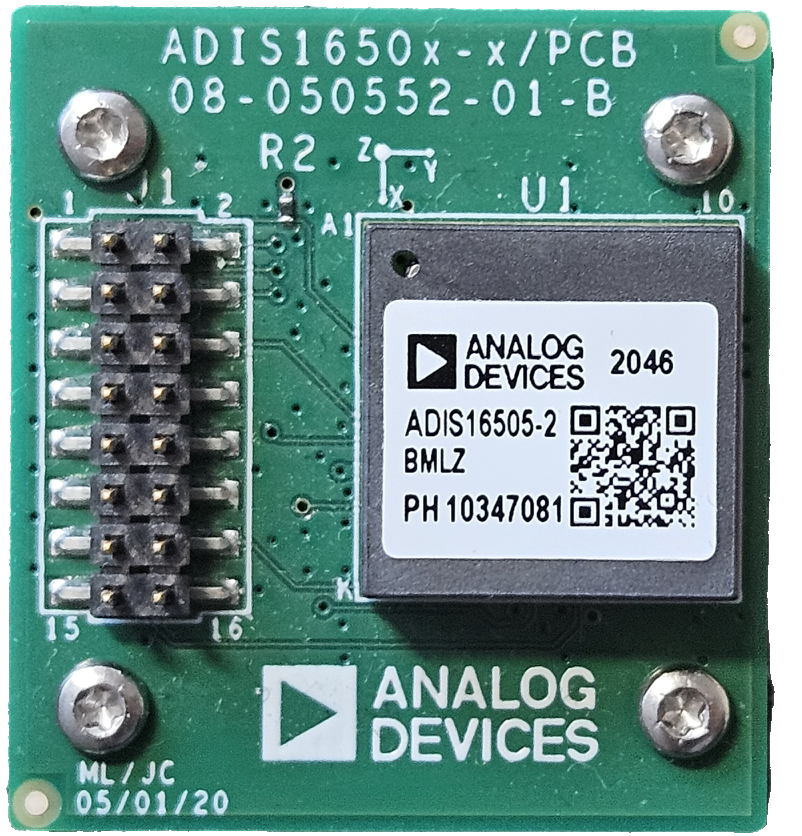
\includegraphics[width=0.4\textwidth]{obrazky/ADIS16505PCB}
    \caption{IMU verze ADIS16505-2/PCBZ.}
    \label{fig:ADIS16505PCB}
\end{figure}

\section{Magnetometr}
Vzhledem k tomu, že výběr komerčně dostupných devítiosých senzorů (akcelerometr, gyroskop a magnetometr) je značně omezený, popřípadě součástky prodávané jako devítiosé IMU jsou ve skutečnosti moduly více součástek na jedné desce, tak je ve výsledném obvodovém zapojení použit senzor magnetické indukce jakožto samostatná součástka. 

Přestože fúze dat z magnetometru může mít pozitivní dopady na zmenšení chyby trajektorie \cite{Tkhorenko2018}, jeho použití uvnitř budov je značně omezené vzhledem k jednoduché ovlivnitelnosti měření blízkými feromagnetickými látkami, silovými rozvody elektřiny a pod. Proto nebyly na výběr magnetometru kladeny vysoké požadavky a slouží spíše pro porovnání vlivu přítomnosti / absence naměřených dat z tohoto senzoru.

K tomuto účelu byl vybrán běžně dostupný obvod LSM303AGR, který kromě magnetometru v pouzdře obsahuje i akcelerometr, ten ovšem nebude pro potřeby práce využit, jelikož tuto funkci obstarávají akcelerometr a gyroskop z kapitoly \ref{AccGyroText}.

Magnetometr komunikuje s hlavním \ac{MCU} přes sběrnici \ac{I2C} s maximální vzorkovací frekvencí 150 Hz, dynamickým rozsahem $ \pm \SI{4.915}{\milli\tesla} $ a 16bitovým rozlišením. \cite{RD5DwZcremhT6bgp}

\section{GNSS}
Zajímavou a uživatelsky přívětivou kombinaci \ac{GNSS} a inerciální navigace poskytuje například firma u-blox s řadou modulů podporující funkci „dead reckoning“. Jedná se o navigační moduly s vestavěným \ac{IMU}, určené zejména do oblasti automobilového průmyslu. Jejich typický příklad použití, dle výrobce, je navigace aut, kdy při běžném provozu je zafixovaný signál z \ac{GNSS} a při výpadku signálu (vjezd do garáže, tunelu apod.) je navigace modulem stále poskytována na základě dat z \ac{IMU}. \cite{DLQg9bT6V1GWKhxh}

Navigační modul u-blox NEO-M8U byl vybrán a implementován do obvodového zapojení inerciální navigační jednotky.
Výrobce udává, že modul zvládne odhadovat polohu po ztrátě signálu \ac{GNSS} po dobu 60 s s typickou odchylkou 10 \% trajektorie. Dále také modul při zapnutí odpovídající funkce umí využít interní \ac{IMU} ke zvýšení maximální rychlosti aktualizace polohy až na 30 Hz. Jeho využití v rámci této práce může být různé, například pro navigaci v místech s alespoň částečným pokrytím signálu \ac{GNSS}. \cite{DLQg9bT6V1GWKhxh}

NEO-M8U umí využívat všechny světové navigační systémy (uvedeny v tabulce~\ref{table:gnssBands})
\begin{table}[h!]
\caption{Podporované družicové systémy. \cite{DLQg9bT6V1GWKhxh} }
\centering
\begin{tabular}{c|c c }

GNSS systém & Pásmo & Frekvence (MHz) \\ 
\hline 
\hline
GPS & L1C/A & 1575,42 \\ 

GLONASS & L1OF & 1602 \\ 

BeiDou & B1 & 1561,098 \\ 

Galileo & E1-B/C & 1575,42 \\ 

\end{tabular} 

\label{table:gnssBands}
\end{table} 

Tento modul komunikuje s hlavním \ac{MCU} přes sběrnici univerzálního asynchronního přijímače-vysílače (\emph{Universal Asynchronous Receiver-Transmitter}, \acsu{UART}), pomocí standardizovaných příkazů americká organizace
námořní elektroniky (\emph{National Marine Electronics Association}, \acsu{NMEA}) příkazů v textové podobě, nebo pomocí binárního protokolu \ac{UBX}, který je specifikován výrobcem. Použití protokolu \ac{NMEA} je omezené pouze na standardní funkce \ac{GNSS} modulů, pokud chceme využít speciálních funkcí, například inerciální navigace, je nutné použít proprietární protokol \ac{UBX}. \cite{DLQg9bT6V1GWKhxh} NEO-M8U také disponuje \ac{USB} portem, skrz který je možné modul ovládat a konfigurovat pomocí PC aplikace výrobce. Tento port je připojen na integrovaný \ac{USB} rozbočovač a lze jej využít například pro vývojové účely.

\section{Paměť}
\begin{table}[h!]
\centering
\begin{tabular}{c|c}

Senzor & Odhadovaný bitrate \\ 
\hline 
\hline 
ADIS16505-2 & 375 kbit/s \\ 

MPU-6050 & 422 kbit/s \\ 

LSM303AGR & 7 kbit/s \\ 

NEO-M8U & 1 kbit/s \\ 
\hline

Celkem & 805 kbit/s (0,1MB/s) \\ 

\end{tabular} 
\caption{Odhad celkového bitratu pro záznam dat} 
\label{table:memoryBW}
\end{table} 
V případě, že bychom chtěli zaznamenávat data ze všech senzorů při jejich maximálních vzorkovacích frekvencích, nebude množství změřených dat zanedbatelné. V tabulce \ref{table:memoryBW} je hrubý odhad potřebné rychlosti záznamu dat pro tento krajní případ. Pokud bude měření trvat např. 2 minuty, vygenerujeme dohromady 12 MB dat, což převyšuje velikost paměti většiny dostupných \ac{MCU}.

Z tohoto důvodu je v obvodovém zapojení inerciální jednotky implementována 32MB NOR Flash paměť, propojená s hlavním \ac{MCU} přes sběrnici QUADSPI s maximální možnou hodinovou frekvencí 120 MHz. Měla by tedy být pro potřeby této aplikace z pohledu velikosti paměti a datového toku dostačující. \cite{CgaRYSTpwKhEZZr7}

Kromě výše popsané Flash paměti jednotka obsahuje i slot na microSD kartu, která by z uživatelského hlediska mohla být jednodušší k použití, ovšem při zápisu může latence SD karty být (krátkodobě) až stovky milisekund. \cite{Kraewinkel2020} To by mohlo znemožnit jejím použití v případě, že by hlavní \ac{MCU} měl nedostatek volné paměti RAM pro krátkodobé uchování dat, proto bude o její využití rozhodnuto až v následujících kapitolách.

\section{Uživatelské rozhraní}
\begin{figure}[h]
    \centering
    \includegraphics[width=0.3\textwidth]{obrazky/OLED}
    \caption{Fotografie grafického OLED displeje.}
\end{figure}
Pro ovládání uživatelem disponuje jednotka grafickým \ac{OLED} displejem s úhlopříčkou 0,96 palce a rozlišením $ 128 \times 64 $ pixelů, který je připojený přes sběrnici \ac{I2C}. Společně s 4 tlačítky by měl poskytnout dostatečně univerzální a pohodlné uživatelské rozhraní.

\section{Napájení} \label{napajeni}
Inerciální jednotka je napájena z jednoho Li-Ion akumulátoru velikosti 18650. Nabíjení je realizováno obvodem BQ24075RGT, který monitoruje nabíjecí odebíraný proud jednotkou. Proud, kterým je nabíjen akumulátor je regulován tak, aby nepřekročil maximální hranici 900 mA z USB portu. \cite{F5eZCtr2LLRsr9NT}

Všechny součásti inerciální jednotky (až na obvod reálného času (\emph{Real Time Clock}, \acsu{RTC}) a zálohovací registry hlavního \ac{MCU} a \ac{GPS} modulu) jsou napájeny skrz DC/DC měnič z výstupního vývodu tohoto nabíjecího obvodu. V případě, že je připojena jednotka do \ac{USB} a nabíjí se, na výstupním pinu nabíjecího obvodu je napájecí napětí USB portu. Díky tomu nedochází k velkým ztrátám pokud je jednotka zapnuta a nabíjí se zároveň. Jestliže je \ac{USB} odpojeno, skrz interní tranzistor je jednotka napájena z akumulátoru. \cite{F5eZCtr2LLRsr9NT}

Nabíjecí obvod také umožňuje kompletní odpojení napájení jednotky přes jeden z vývodů. Toho je využito pro ochranu akumulátoru proti podvybití pomocí zapojení S/R klopného obvodu na napájení \ac{USB} a jednoho z výstupů procesoru. Napětí akumulátoru je měřeno pomocí \ac{ADC} mikrokontroléru. Jestliže klesne pod definovanou úroveň, pomocí pulzu bude celý obvod odpojen od napájení až do té doby, dokud uživatel znovu nepřipojí jednotku do \ac{USB} portu.

\begin{table}[h!]
\centering

\begin{tabular}{|c|c|}
\hline 
Součástka & Odhadovaný proud (mA) \\ 
\hline 
\hline 
STM32F446 & 50 \\ 
\hline 
ESP32 & 150 \\ 
\hline 
USB2514 & 135 \\ 
\hline 
ADIS16505 & 50 \\ 
\hline 
NEO-M8U & 30 \\ 
\hline 
OLED displej & 10 \\ 
\hline 
microSD karta & 50 \\ 
\hline 
\hline 
Celkem & 475 \\ 
\hline 
\end{tabular} 

\caption{Odhad spotřeby proudu 3,3V větve} 
\label{table:currentConsumption}
\end{table} 

Vzhledem k většímu počtu součástek není odebíraný proud z 3,3V napájecí větve malý (zhruba 0,5 A, viz. tabulka \ref{table:currentConsumption}). Budeme-li uvažovat rozsah výstupního napětí nabíjecího obvodu 3,5 V (vybitý akumulátor) až 5 V (zařízení připojené do \ac{USB}) zjistíme, že pro napájení 3,3V větve není vhodný lineární regulátor, zejména kvůli vysokému ztrátovému výkonu. Ten je v krajním případě

\begin{equation}
P_{\mathrm{ztrátový}} = (U_{\mathrm{USB}}-U_{\mathrm{IO}})\cdot I_{\mathrm{IO}}=(5-3,3)\cdot 0,5= \SI{0,85}{\watt} .
\end{equation}

Proto byl na napájení hlavní 3,3V větve vybrán spínaný regulátor TPS62823. Jedná se o buck (snižující) měnič s integrovaným výkonovým tranzistorem pracujícím na frekvenci 2,2 MHz. Díky vyšší spínací frekvenci je možné využít menší komponenty, zejména cívku a filtrační kondenzátory na výstup, ovšem je potřeba dodržet doporučovaná pravidla při návrhu desky pro omezení rušení a velkých proudových smyček. Rozsah napájecího napětí čipu je 2,4 až 5 V, maximální výstupní proud 3 A. \cite{mGnys3WmOkWuaQHN}

Minimální napětí, na které můžeme nechat akumulátor vybít je dáno odpory přechodů Drain-Source vnitřních tranzistorů nabíjecího obvodu, DC/DC měniče a stejnosměrným odporem cívky. V tomto případě bude regulátor pracovat v módu s minimální střídou. \cite{mGnys3WmOkWuaQHN} Toto napětí je
\begin{equation}
\begin{matrix}
 U_{\mathrm{batMin}} = U_{\mathrm{out}} + I_{\mathrm{out}} \cdot (R_{\mathrm{DS(charge)}} + R_{\mathrm{DS(conv)}} + R_{\mathrm{DC(L)}})= \\
  =3,3 + 0,5 \cdot (0,05 + 0,026 + 0,014) = \SI{3,345}{\volt}
\end{matrix} .
 \end{equation}

\section{Hlavní procesor}
Požadavky na výběr hlavního procesoru byly z velké části dané počtem a druhem potřebných periferií, které jsou popsané v tabulce \ref{table:MCUperiferie}.
Dále byly z podskupiny procesorů disponujících všemi periferiemi z tabulky \ref{table:MCUperiferie} vybrány takové, které mají velikost vnitřní FLASH paměti alespoň 512 kB, abychom nebyli při vývoji Firmwaru jednotky omezeni velikostí programu. Pouzdra procesorů byla vybrána taková, aby se s nimi dalo jednoduše pracovat, z toho důvodu byla vyloučena pouzdra typu \ac{BGA}. 
V neposlední řadě byla zvážena i dostupnost vybíraných procesorů u nejobvyklejších distributorů elektronických součástek, aby bylo možné v případě potřeby výrobu jednotky opakovat.

\begin{table}[ht]
\centering
\begin{tabular}{|c|c|c|}
\hline 
Druh periferie & Minimální požadovaný počet & Použití periferie \\ 
\hline 
\hline 
I2C & 3 & \makecell{OLED displej, LSM303AGR, \\MPU6050, USB2514B}  \\ 
\hline 
SPI & 1 & ADIS16505 \\ 
\hline 
UART & 2 & NEO-M8U, ESP32 \\ 
\hline 
QUADSPI & 1 & NOR FLASH paměť \\ 
\hline 
SDIO & 1 & microSD karta \\ 
\hline 
ADC & 1 & měření napětí akumulátoru \\ 
\hline 
\end{tabular} 

\caption{Minimální požadavky na periferie mikroprocesoru.} 
\label{table:MCUperiferie}
\end{table} 


Na základě těchto požadavků byl vybrán mikrokontrolér \emph{STM32F446VET6}. Jedná se o 32bitový ARM Cortex-M4 procesor z portfolia „high performance“ mikrokontrolérů výrobce STMicroelectronics. Splňuje všechny výše zmíněné minimální požadavky, v obvodovém zapojení byla použita i USB periferie procesoru, která může mít různá využití. Procesor obsahuje 512 kB paměti Flash a 128 kB paměti RAM, maximální hodinová frekvence je 180 MHz a disponuje matematickým koprocesorem pro operace s plovoucí desetinou čárkou. Vzhledem k počtu univerzálních vstupních/výstupních pinů (\emph{General Purpose Input/
Output}, \acsu{GPIO}) v zapojení inerciální jednotky byla vybrána varianta procesoru v pouzdře LQFP100. \cite{csdGtKJDMSdbwJ9r}

\section{ESP32}
Pro splnění požadavků zadání práce je potřeba, aby mohla inerciální jednotka komunikovat bezdrátově s PC zpracovávajícím data. Pro tento úkol byl vybrán bezdrátový modul ESP32-C3-Mini. Jedná se o jeden z novějších produktů portfolia bezdrátových modulů firmy Espressif. Podporuje standard WiFi 802.11 b/g/n a Bluetooth~LE~5. \cite{zJ7x5ye8Y5eJn1E2}

Tento modul je v obvodovém zapojení použit čistě jako bezdrátové rozhraní, neobsluhuje žádné další \ac{GPIO} kromě 2 \ac{UART} sběrnic. První sběrnice \ac{UART} je připojena pomocí USB-serial převodníku CH340 na \ac{USB} rozbočovač v inerciální jednotce. Toto rozhraní slouží pro nahrávání, popřípadě aktualizaci vestavěného AT firmwaru výrobce. V případě, že by poskytovaný firmware výrobce nedostačoval, nebo nebyl vhodný pro potřeby naší aplikace, bude možné pomocí tohoto rozhraní nahrát vlastní obslužný firmware pro ESP32.

Druhá sběrnice \ac{UART} je připojena k hlavnímu \ac{MCU} inerciální jednotky. Kromě standardních pinů Rx a Tx jsou propojeny i piny pro řízení toku, které by bylo možné použít na zjednodušení časování komunikace.

\section{Testování s vývojovými stavebnicemi}
Pro účely vyzkoušení fúze dat z \ac{GNSS} modulu a inerciálních senzorů byl navržen 3D tištěný držák (na obrázku \ref{fig:devBoards}) pro upevnění vývojových stavebnic osazených NEO-M8U a ADIS16505 s potřebnými periferními obvody na připojení k PC přes \ac{USB}. Pomocí skriptů v Pythonu je možné ukládat data z obou senzorů do csv souborů a ty následně spojit.

Vzhledem k asynchronnosti \ac{USB} komunikace bylo složité udržet definované vzorkovací kmitočty, popřípadě vzorkovat data z \ac{GNSS} a \ac{IMU} zároveň. Z tohoto důvodu byly desky použity na základní otestování a rozsáhlejší zpracování dat bude provedeno až s vlastní deskou hardwaru popsaném v kapitole \ref{hardware}.
\begin{figure}[h] 
    \centering
    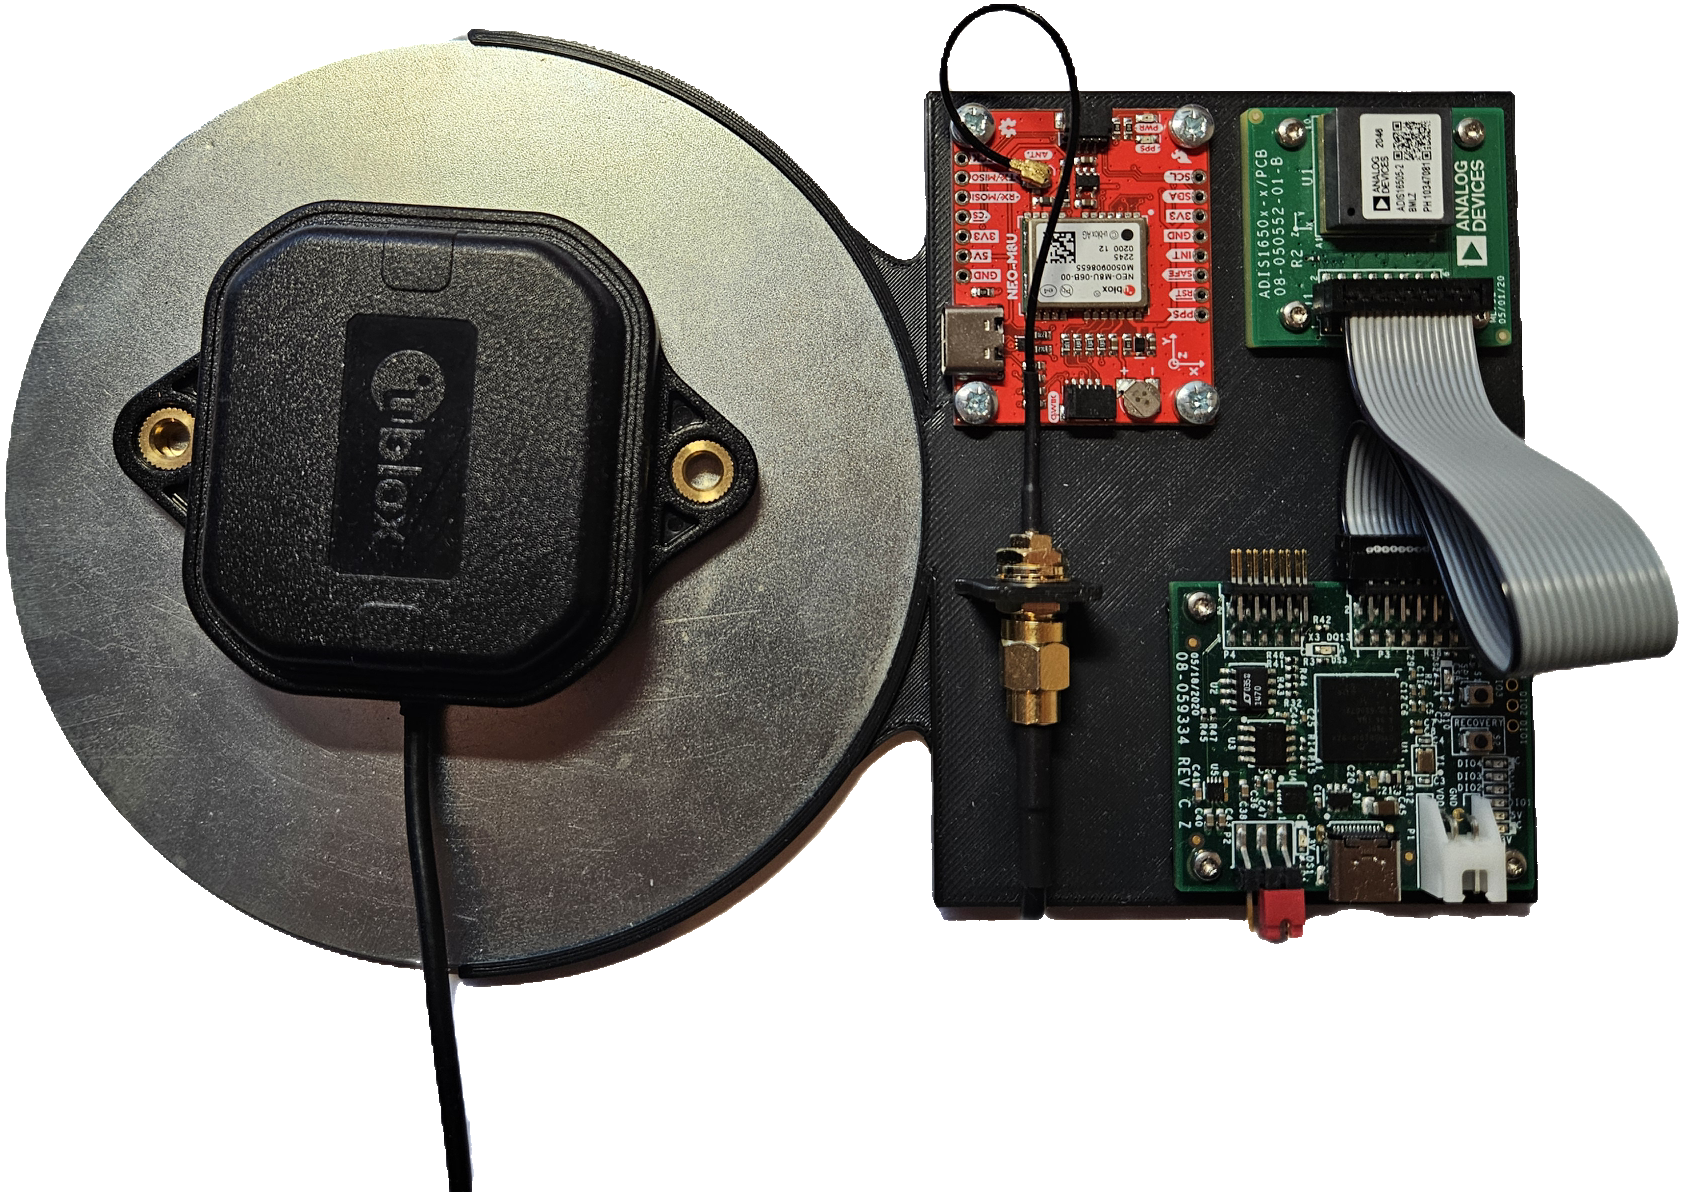
\includegraphics[width=0.9\textwidth]{obrazky/devBoards}
    \caption{Testovací přípravek s vývojovými deskami.}
    \label{fig:devBoards}
\end{figure}

\chapter{Realizace hardwaru} \label{hardware}
\begin{figure}[h]
    \centering
    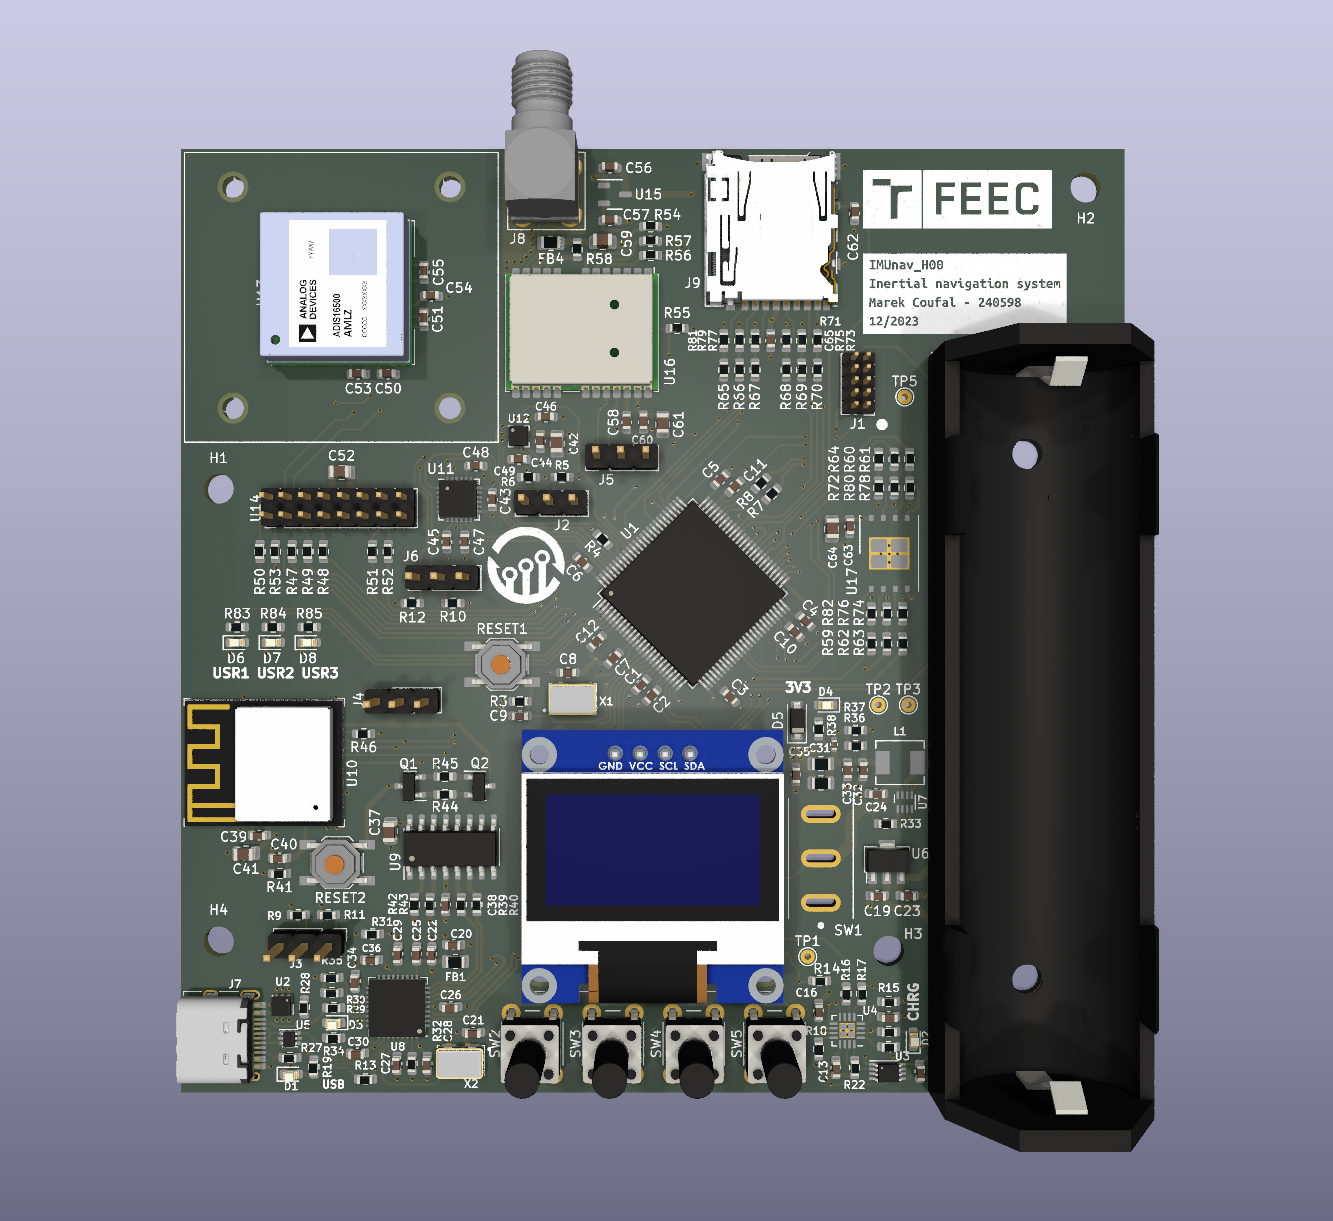
\includegraphics[width=\textwidth]{KiCad/3Dboard}
    \caption{3D model navržené DPS.}
    \label{fig:3Dboard}
\end{figure}

Schéma i \ac{DPS} byly navrženy v programu KiCad. V příloze \ref{schemaApp} je schéma inerciální jednotky rozdělené do několika logických bloků. Příloha \ref{placementApp} obsahuje pohled na osazení součástek vrchní vrstvy a přílohy \ref{TopApp} až \ref{BottomApp} obsahují nákres jednotlivých vrstev mědi. Na obrázku \ref{fig:3Dboard} je vygenerovaný 3D model \ac{DPS}. Celý projekt programu KiCad je také dostupný v elektronické příloze.

Inerciální jednotka je realizována jako čtyřvrstvá deska plošných spojů o velikosti $ 100 \times 100 $ mm s uspořádáním vrstev popsaném v tabulce \ref{table:signalStackup}.
\begin{table}[h!]
\caption{Signálové uspořádání vrstev na DPS.} 
\centering

\begin{tabular}{|c|c|}
\hline 
Vrstva mědi & Využití \\ 
\hline 
\hline 
Horní & Vysokorychlostní signály \\ 
\hline 
1. vnitřní & Společná zem \\ 
\hline 
2. vnitřní & Napájení \\ 
\hline 
Dolní & Signály \\ 
\hline 
\end{tabular} 


\label{table:signalStackup}
\end{table} 

Typ a tloušťka substrátu \ac{DPS} byla vybrána v konfiguraci JLC04161H-7628, jejich mechanické uspořádání a dielektrické vlastnosti jsou popsané v tabulce \ref{table:materialStackup}. Pomocí kalkulačky výrobce byly vypočteny potřebné hodnoty požadovaných šířek a mezer spojů mikropáskového vedení pro impedanci \SI{50}{\ohm} a \SI{90}{\ohm}. Hodnoty pro vedení o impedanci \SI{50}{\ohm} byly použity při návrhu cest mezi \ac{GPS} modulem a anténo subminiaturní verze A (\emph{Sub-
Miniature version A}, \acsu{SMA}). Šírka a vzdálenost diferenciálního páru o impedanci \SI{90}{\ohm} byla použita při návrhu \ac{USB} části zapojení.
\begin{table}[ht]
\centering

\begin{tabular}{|c|c|c|}
\hline 
Typ materiálu & Tloušťka (mm) & Relativní permitivita $ \epsilon_{r} $(-) \\ 
\hline 
\hline 
Vrchní vrstva mědi & 0,0350 & 1 \\ 
\hline 
Prepreg 7628 & 0,2104 & 4,4 \\ 
\hline 
1. vnitřní vrstva mědi & 0,0152 & 1 \\ 
\hline 
Jádro & 1,065 & 4,6 \\ 
\hline 
2. vnitřní vrstva mědi & 0,0152 & 1 \\ 
\hline 
Prepreg 7628 & 0,2104 & 4,4 \\ 
\hline 
Spodní vrstva mědi & 0,0350 & 1 \\ 
\hline 
\end{tabular} 

\caption{Uspořádání měděných a izolačních vrstev DPS JLC04161H-7628} 
\label{table:materialStackup}
\end{table} 


Většina pouzder pasivních součástek byla vybrána o velikosti 0603, což by mělo poskytnout dostatečný kompromis mezi velikostí výsledné desky a možností ruční výměny součástky pro případné opravy na prvním prototypu. Prototypová deska je také opatřena měřícími body na napájecích větvích a konektorovými hřebínky na digitálních komunikacích pro možnost připojení osciloskopu, nebo logického analyzátoru na odposlouchávání komunikace mezi \ac{MCU} a jednotlivými senzory. 

\section{Konstrukce}

Všechny SMD součástky, kromě \ac{GNSS} a \ac{IMU} modulu byly osazeny strojově, zbylé součástky a konstrukční prvky ručně. Vzhledem k tomu, že deska byla navržena pro možnost výběru použití BGA, nebo PCB varianty ADIS16505, tak v případě použití hotového modulu je potřeba použít izolační desku, která zamezí nežádoucím zkratům mezi odkrytými ploškami neosazeného BGA pouzdra a PCB varianty inerciálního modulu. K tomuto účelu byl navržen jednoduchý 3D tištěný izolační prvek, který je vložen mezi jednotlivé desky, znázorněn na obrázku \ref{fig:adisIsolator}.

\begin{figure}
     \centering
     \begin{subfigure}[b]{0.45\textwidth}
         \centering
         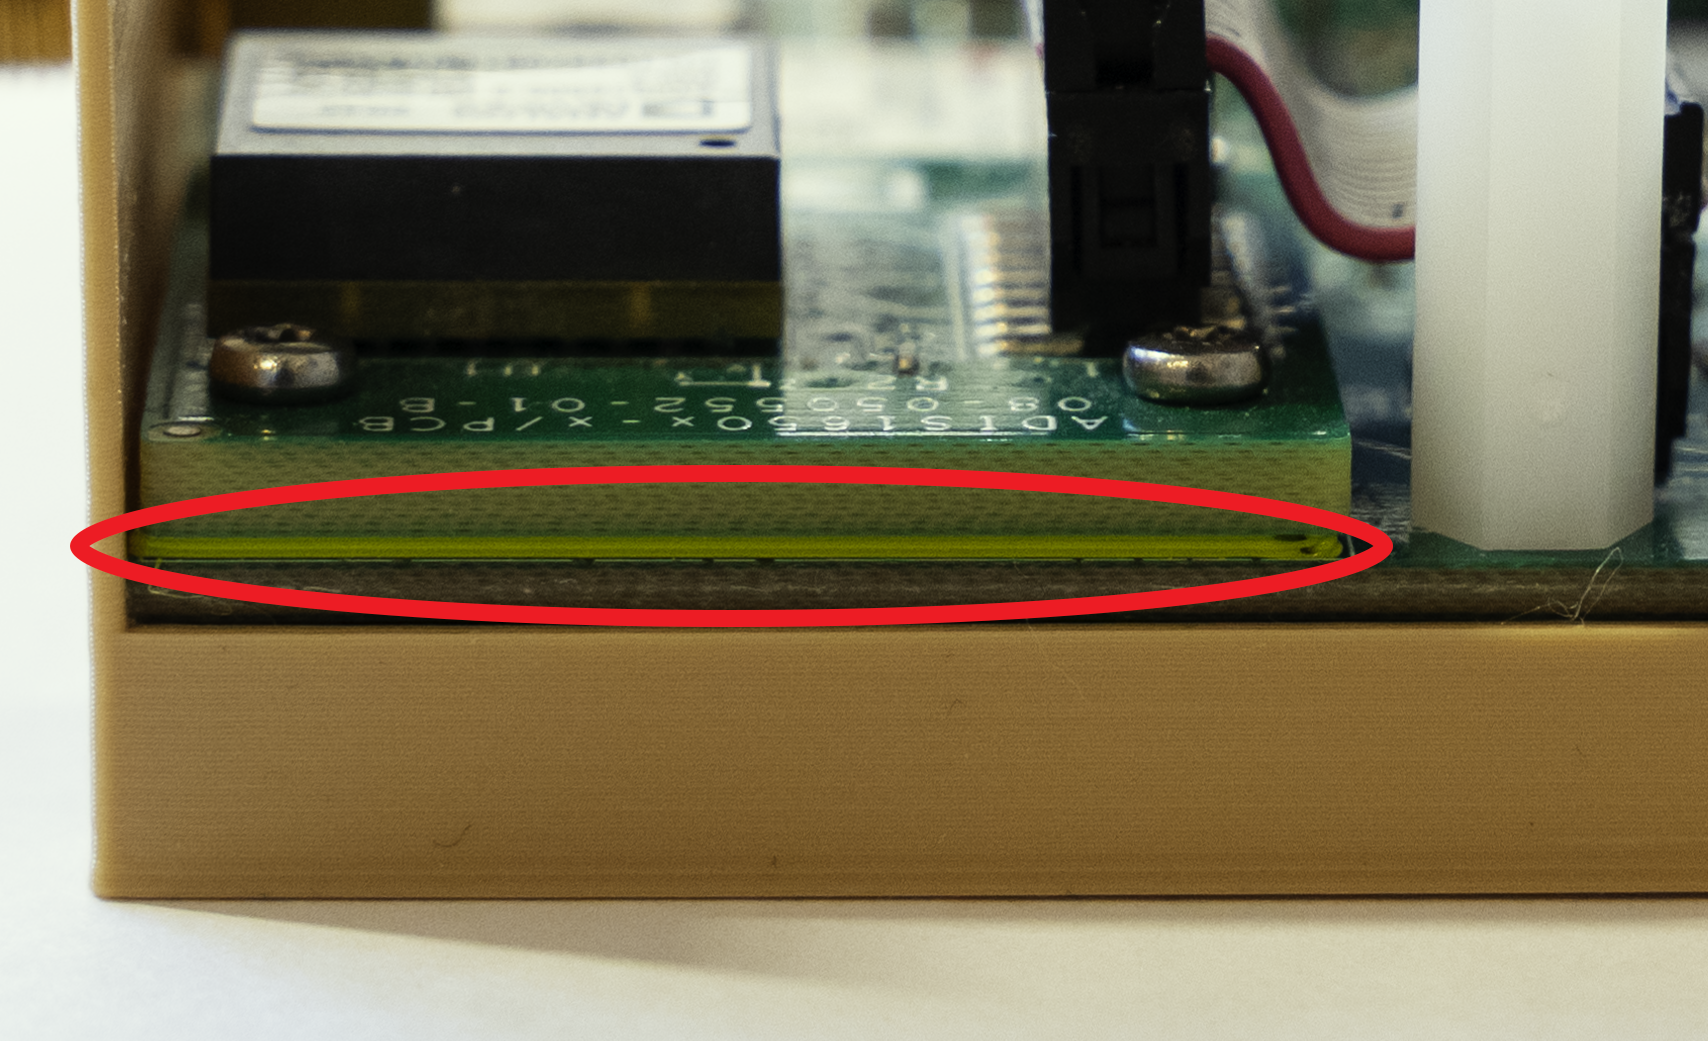
\includegraphics[width=\textwidth]{obrazky/isolatorADIS}
         \caption{Fotografie umístěného izolátoru.}
       
     \end{subfigure}
     \hfill
     \begin{subfigure}[b]{0.45\textwidth}
         \centering
         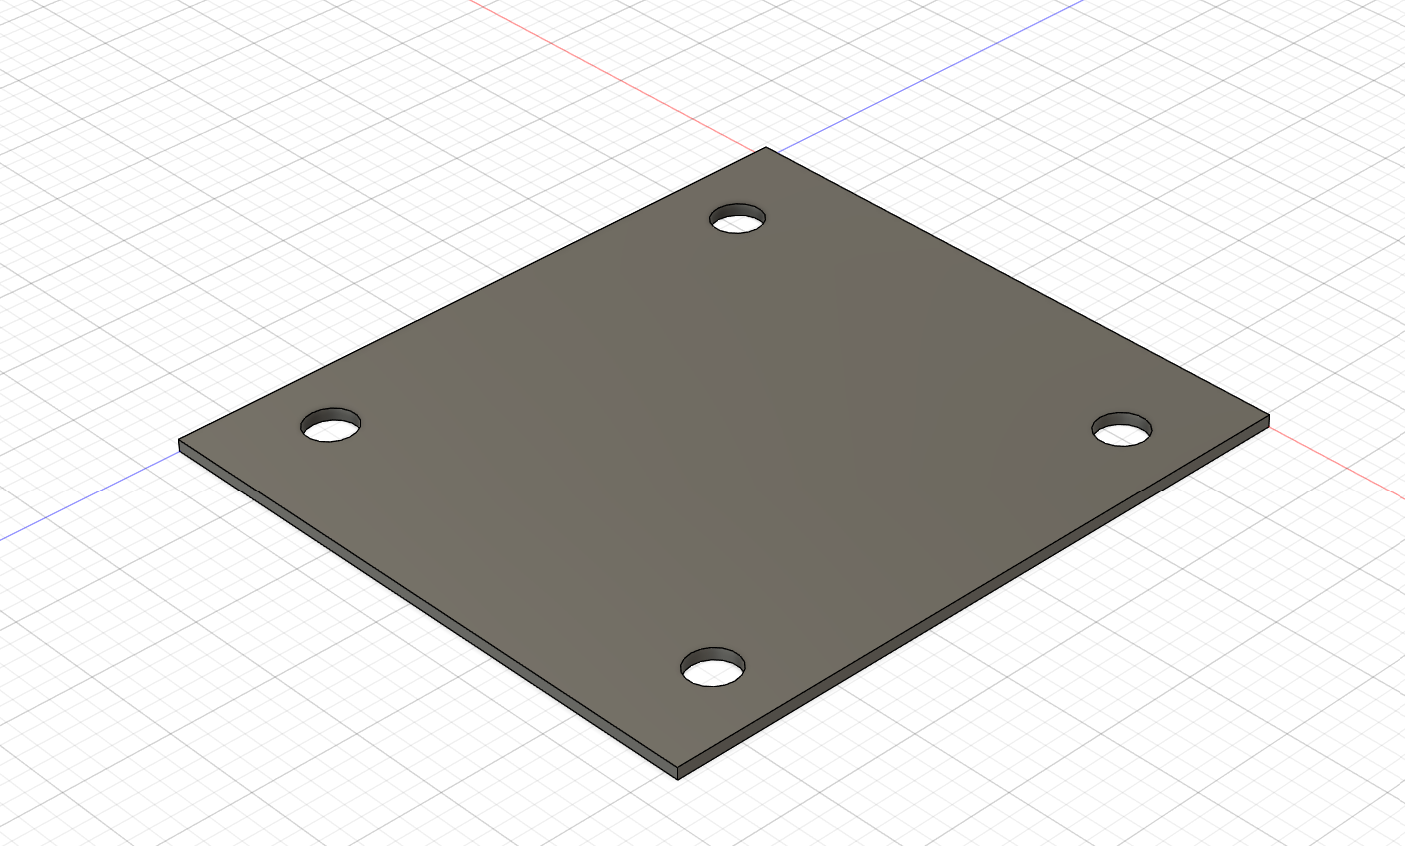
\includegraphics[width=\textwidth]{obrazky/ModelIsolatorADIS}
         \caption{3D model izolátoru.}
         
     \end{subfigure}
        \caption{Izolační podložka IMU.}
        \label{fig:adisIsolator}
\end{figure}

Obdobné izolační podložky byly také navrženy a použity při montáži distančních sloupků držící \ac{OLED} displej.

\begin{figure}
     \centering
     \begin{subfigure}[b]{0.45\textwidth}
         \centering
         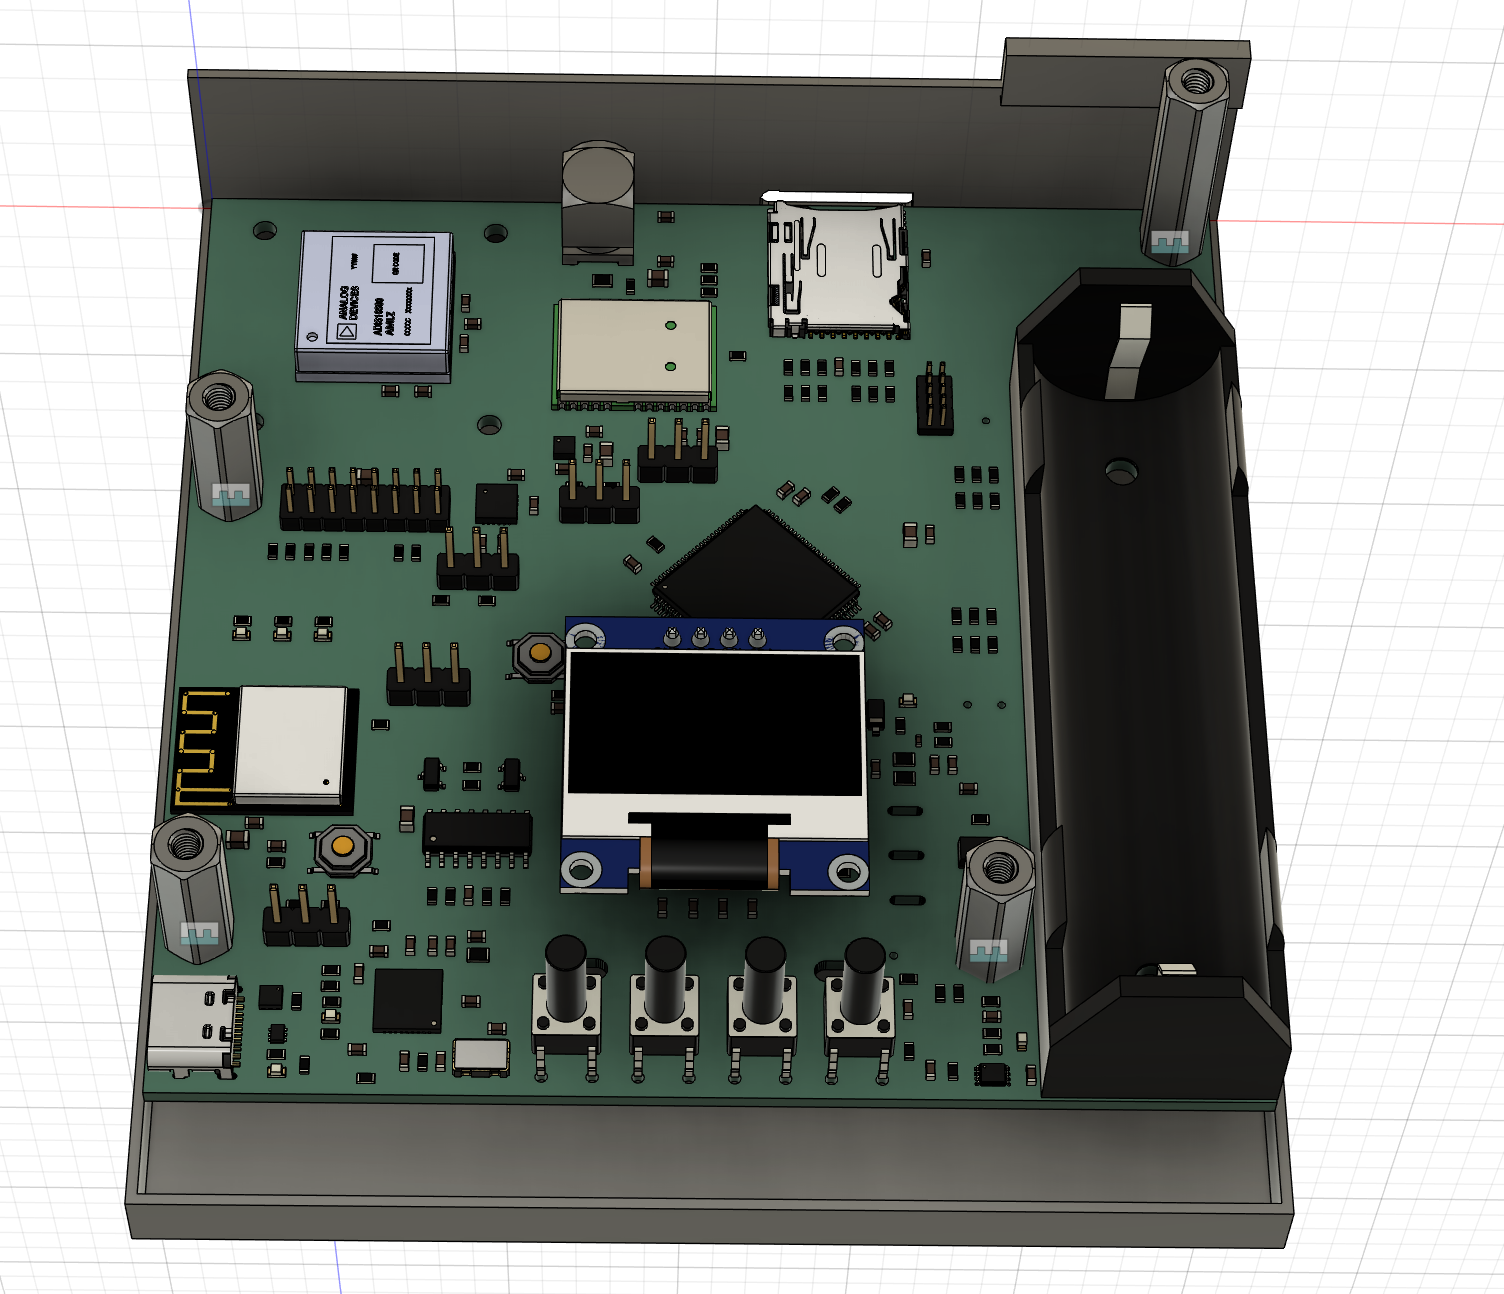
\includegraphics[width=\textwidth]{obrazky/boxNoLid}
         \caption{3D model krabičky bez víka.}
       
     \end{subfigure}
     \hfill
     \begin{subfigure}[b]{0.45\textwidth}
         \centering
         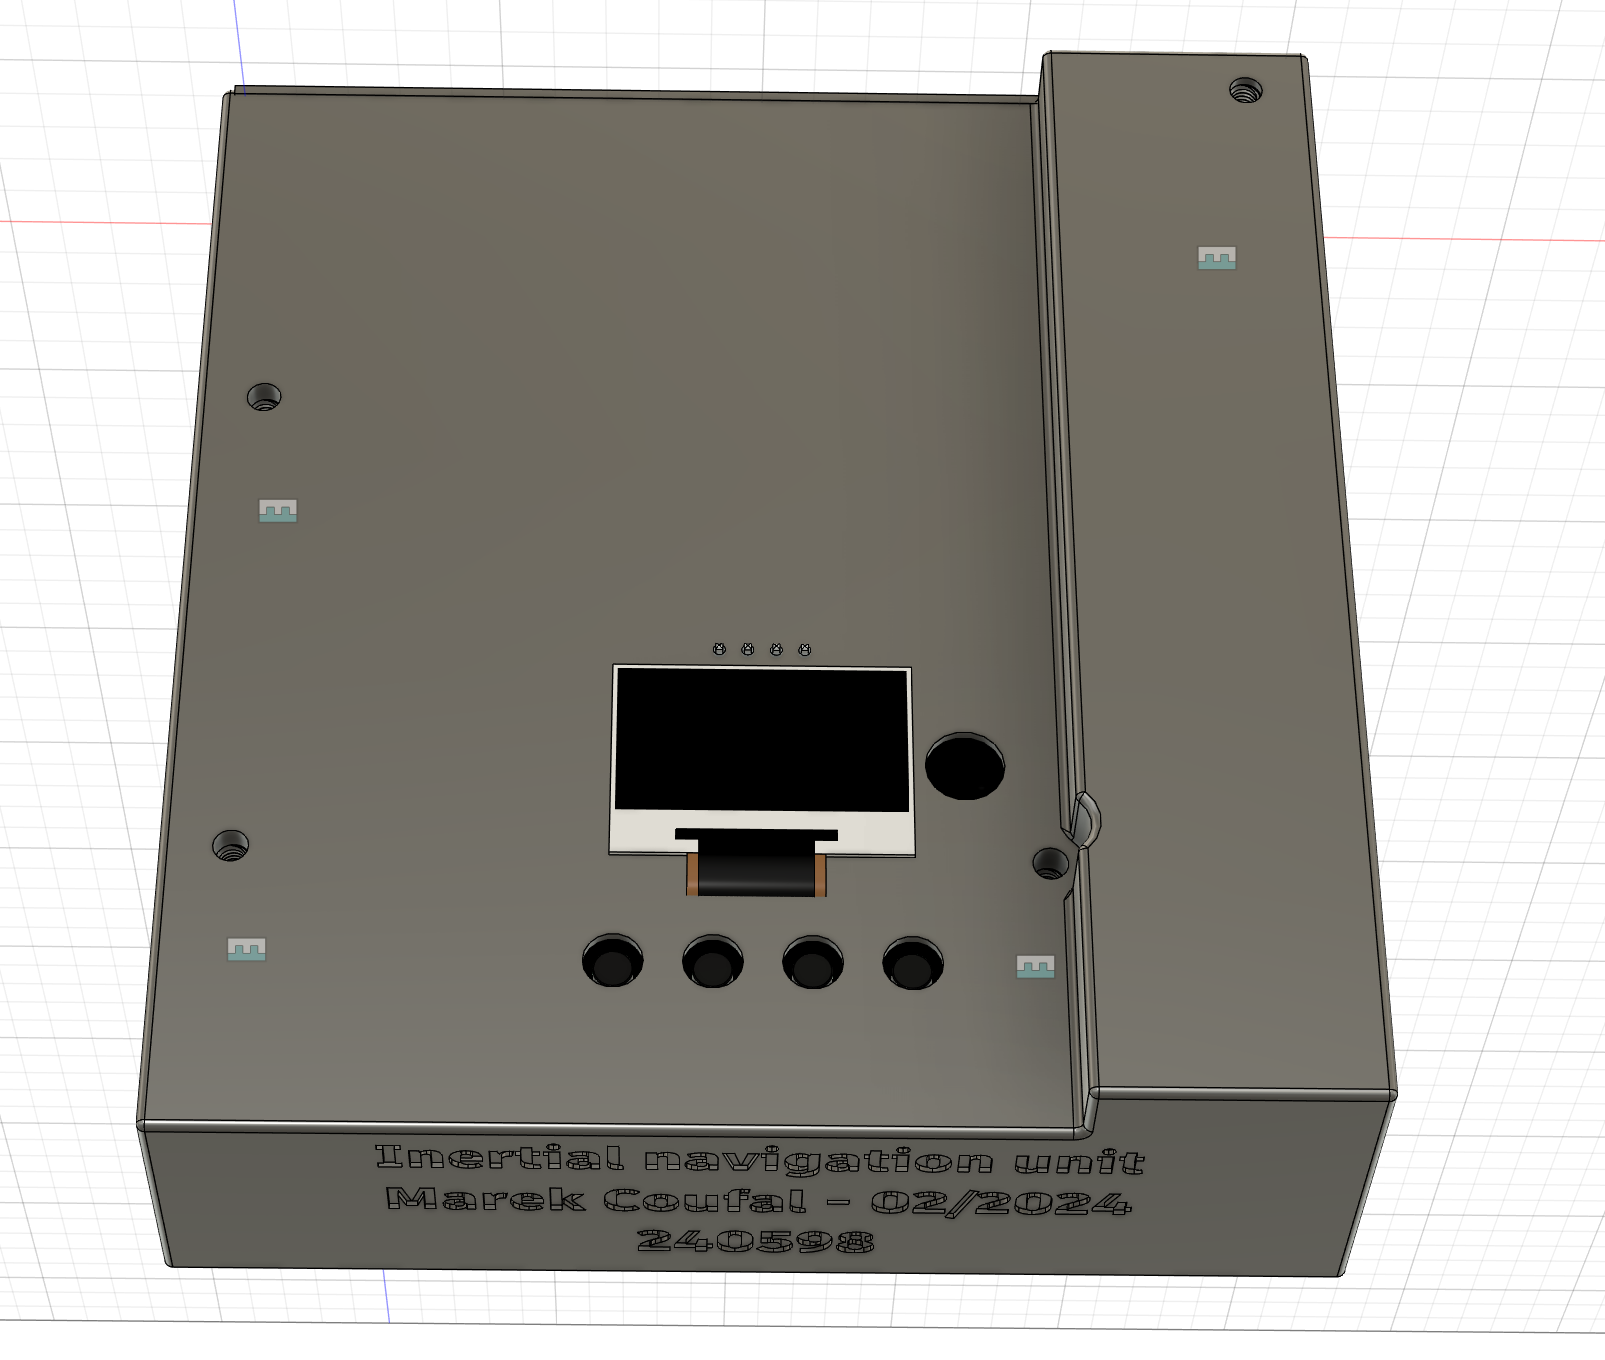
\includegraphics[width=\textwidth]{obrazky/boxWithLid}
         \caption{3D model krabičky s víkem.}
         
     \end{subfigure}
        \caption{3D model krabičky.}
        \label{fig:boxModel}
\end{figure}

Dále byla navržena a vyrobena 3D tištěná montážní krabička (obrázek \ref{fig:boxModel}) pro ochranu citlivých komponent zařízení při běžném užívání a manipulaci. Veškeré modely v této práci jsou navrženy pomocí 3D počítačem podporovanému
projektovacímu (\emph{Computer-Aided Design}, \acsu{CAD}) programu Fusion 360 od firmy Autodesk. Ve spodní části krabičky jsou přidané závitové vložky, které byly teplem vlisovány do plastového dílu pomocí mikropájky. \ac{DPS} je připevněna k tomuto dílu pomocí čtveřice nylonových distančních sloupků, které zároveň slouží jako vzpěry pro vrchní díl krabice. Sestavené zařízení je na obrázku \ref{fig:boxPhoto}.

\begin{figure}
     \centering
     \begin{subfigure}[b]{0.4\textwidth}
         \centering
         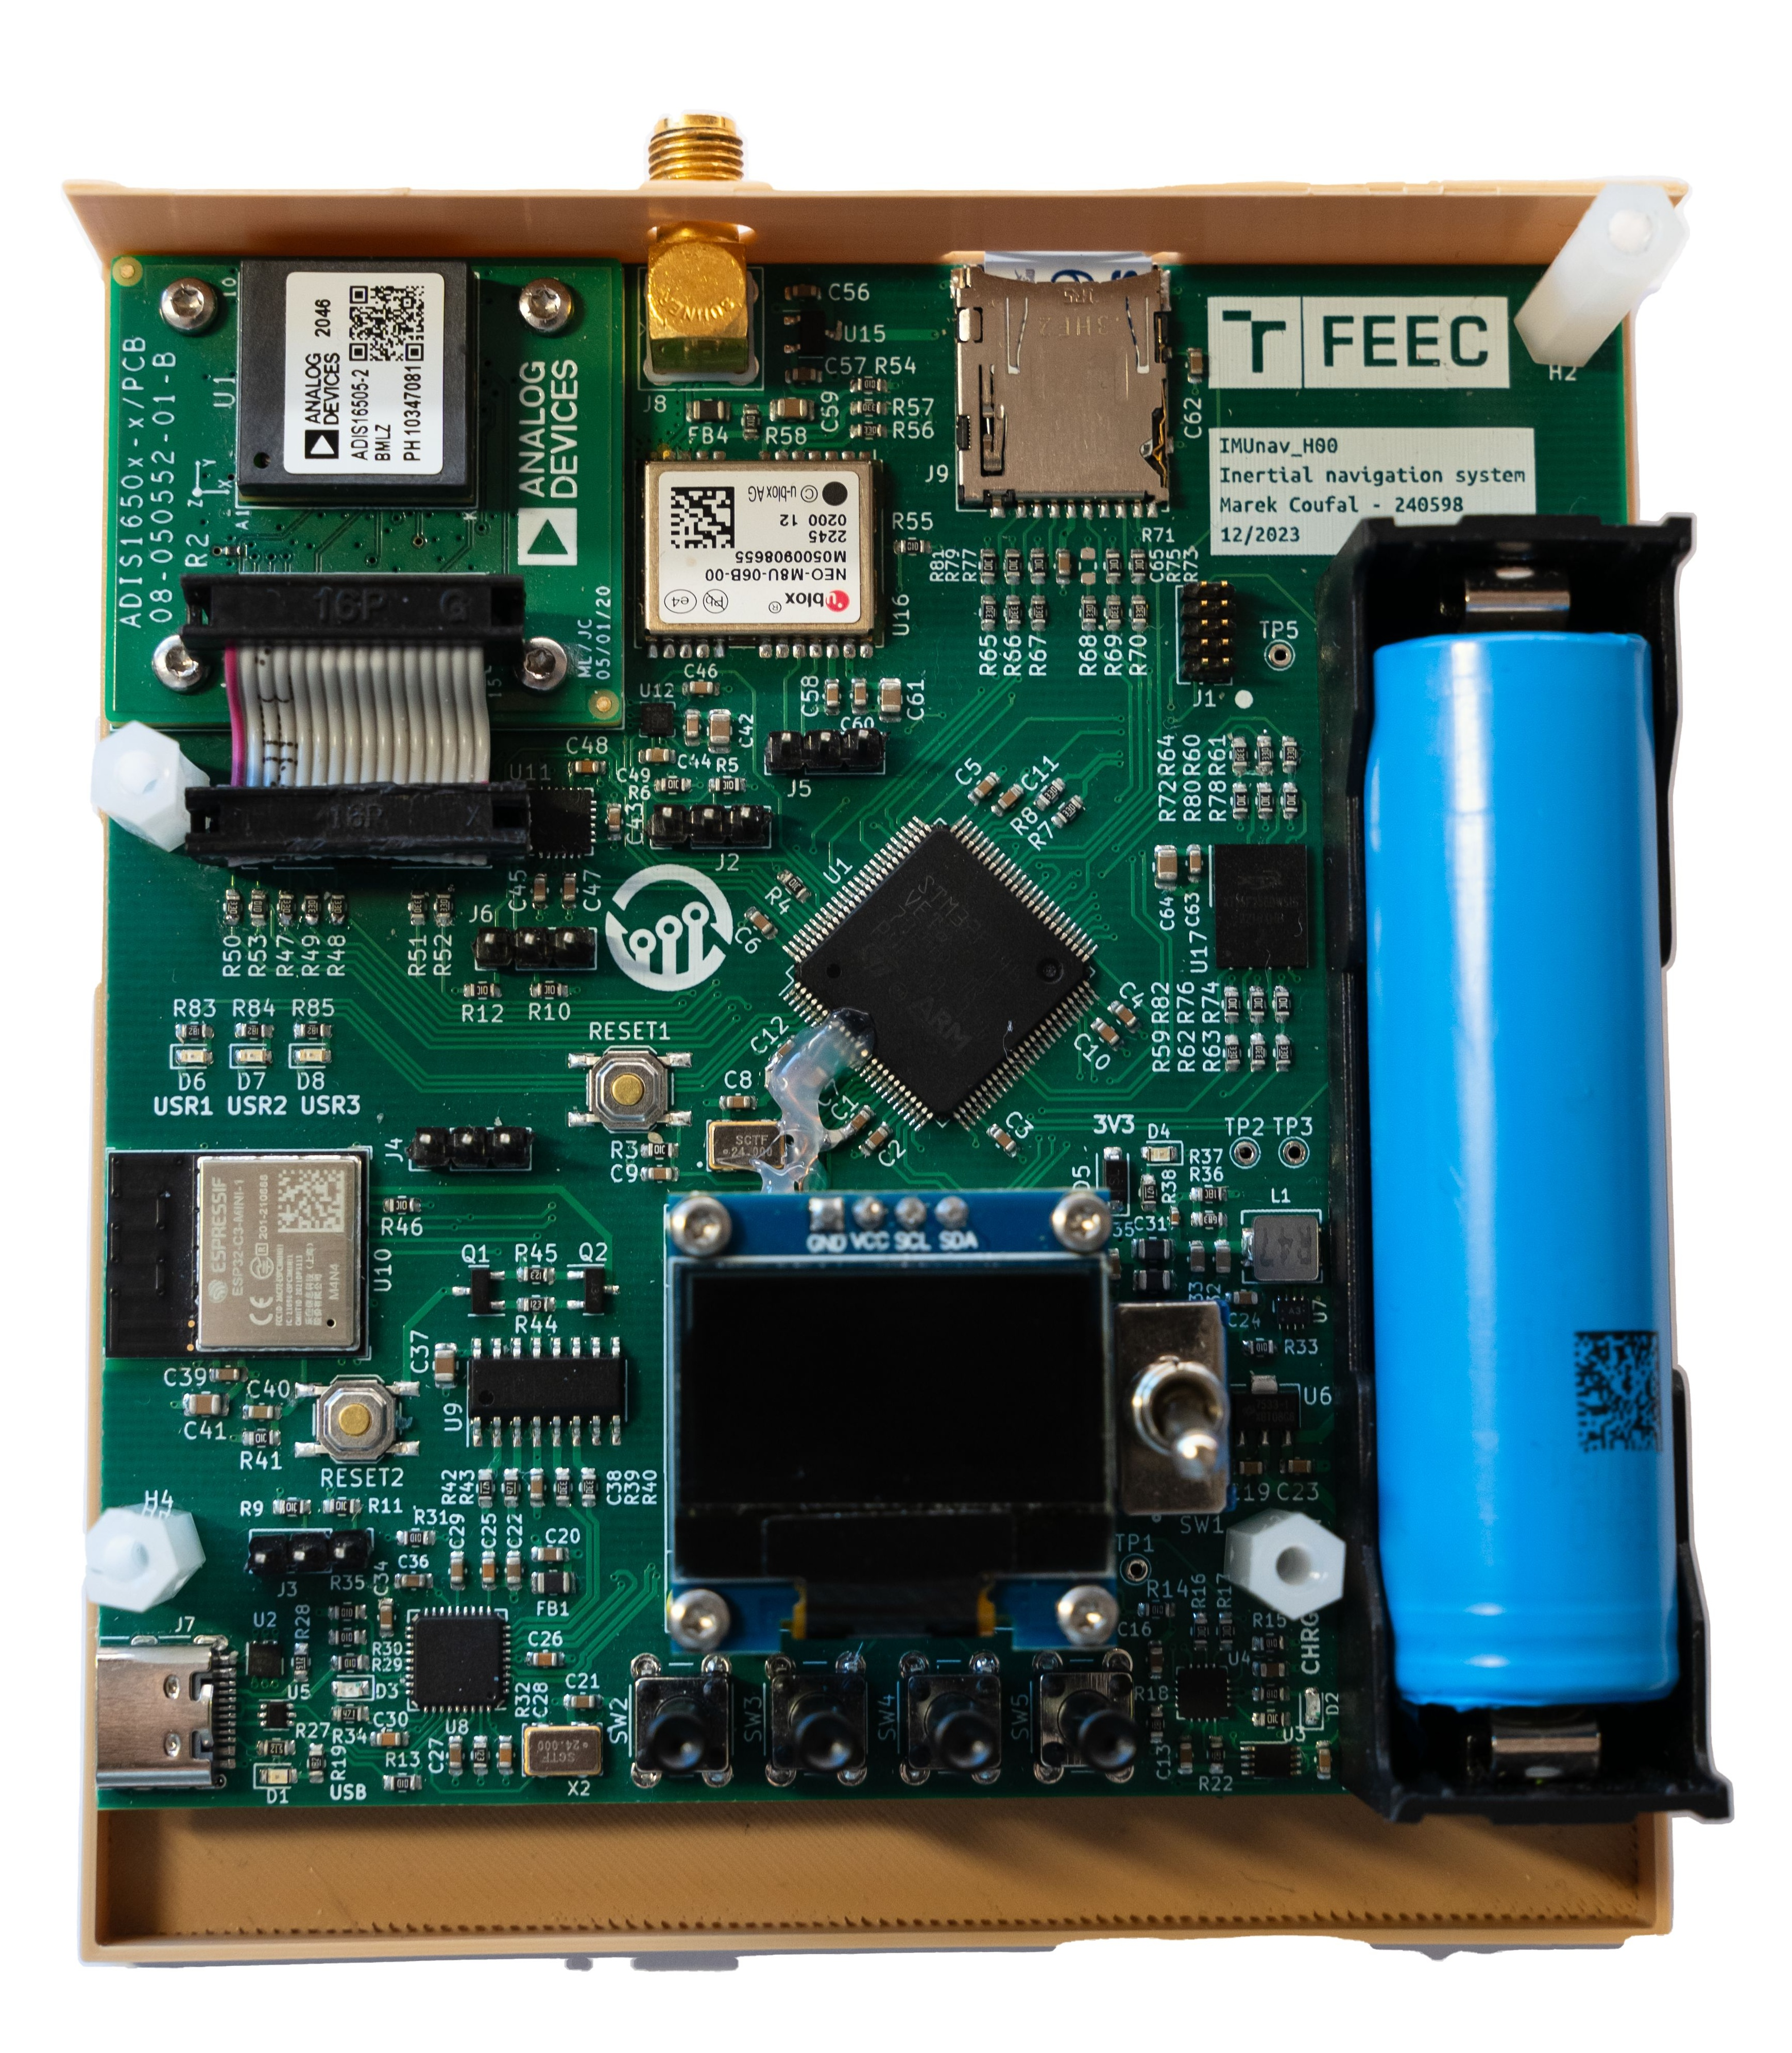
\includegraphics[width=\textwidth]{obrazky/imuNavPCB}
         \caption{Spodní díl krabičky s deskou.}
       
     \end{subfigure}
     \hfill
     \begin{subfigure}[b]{0.4\textwidth}
         \centering
         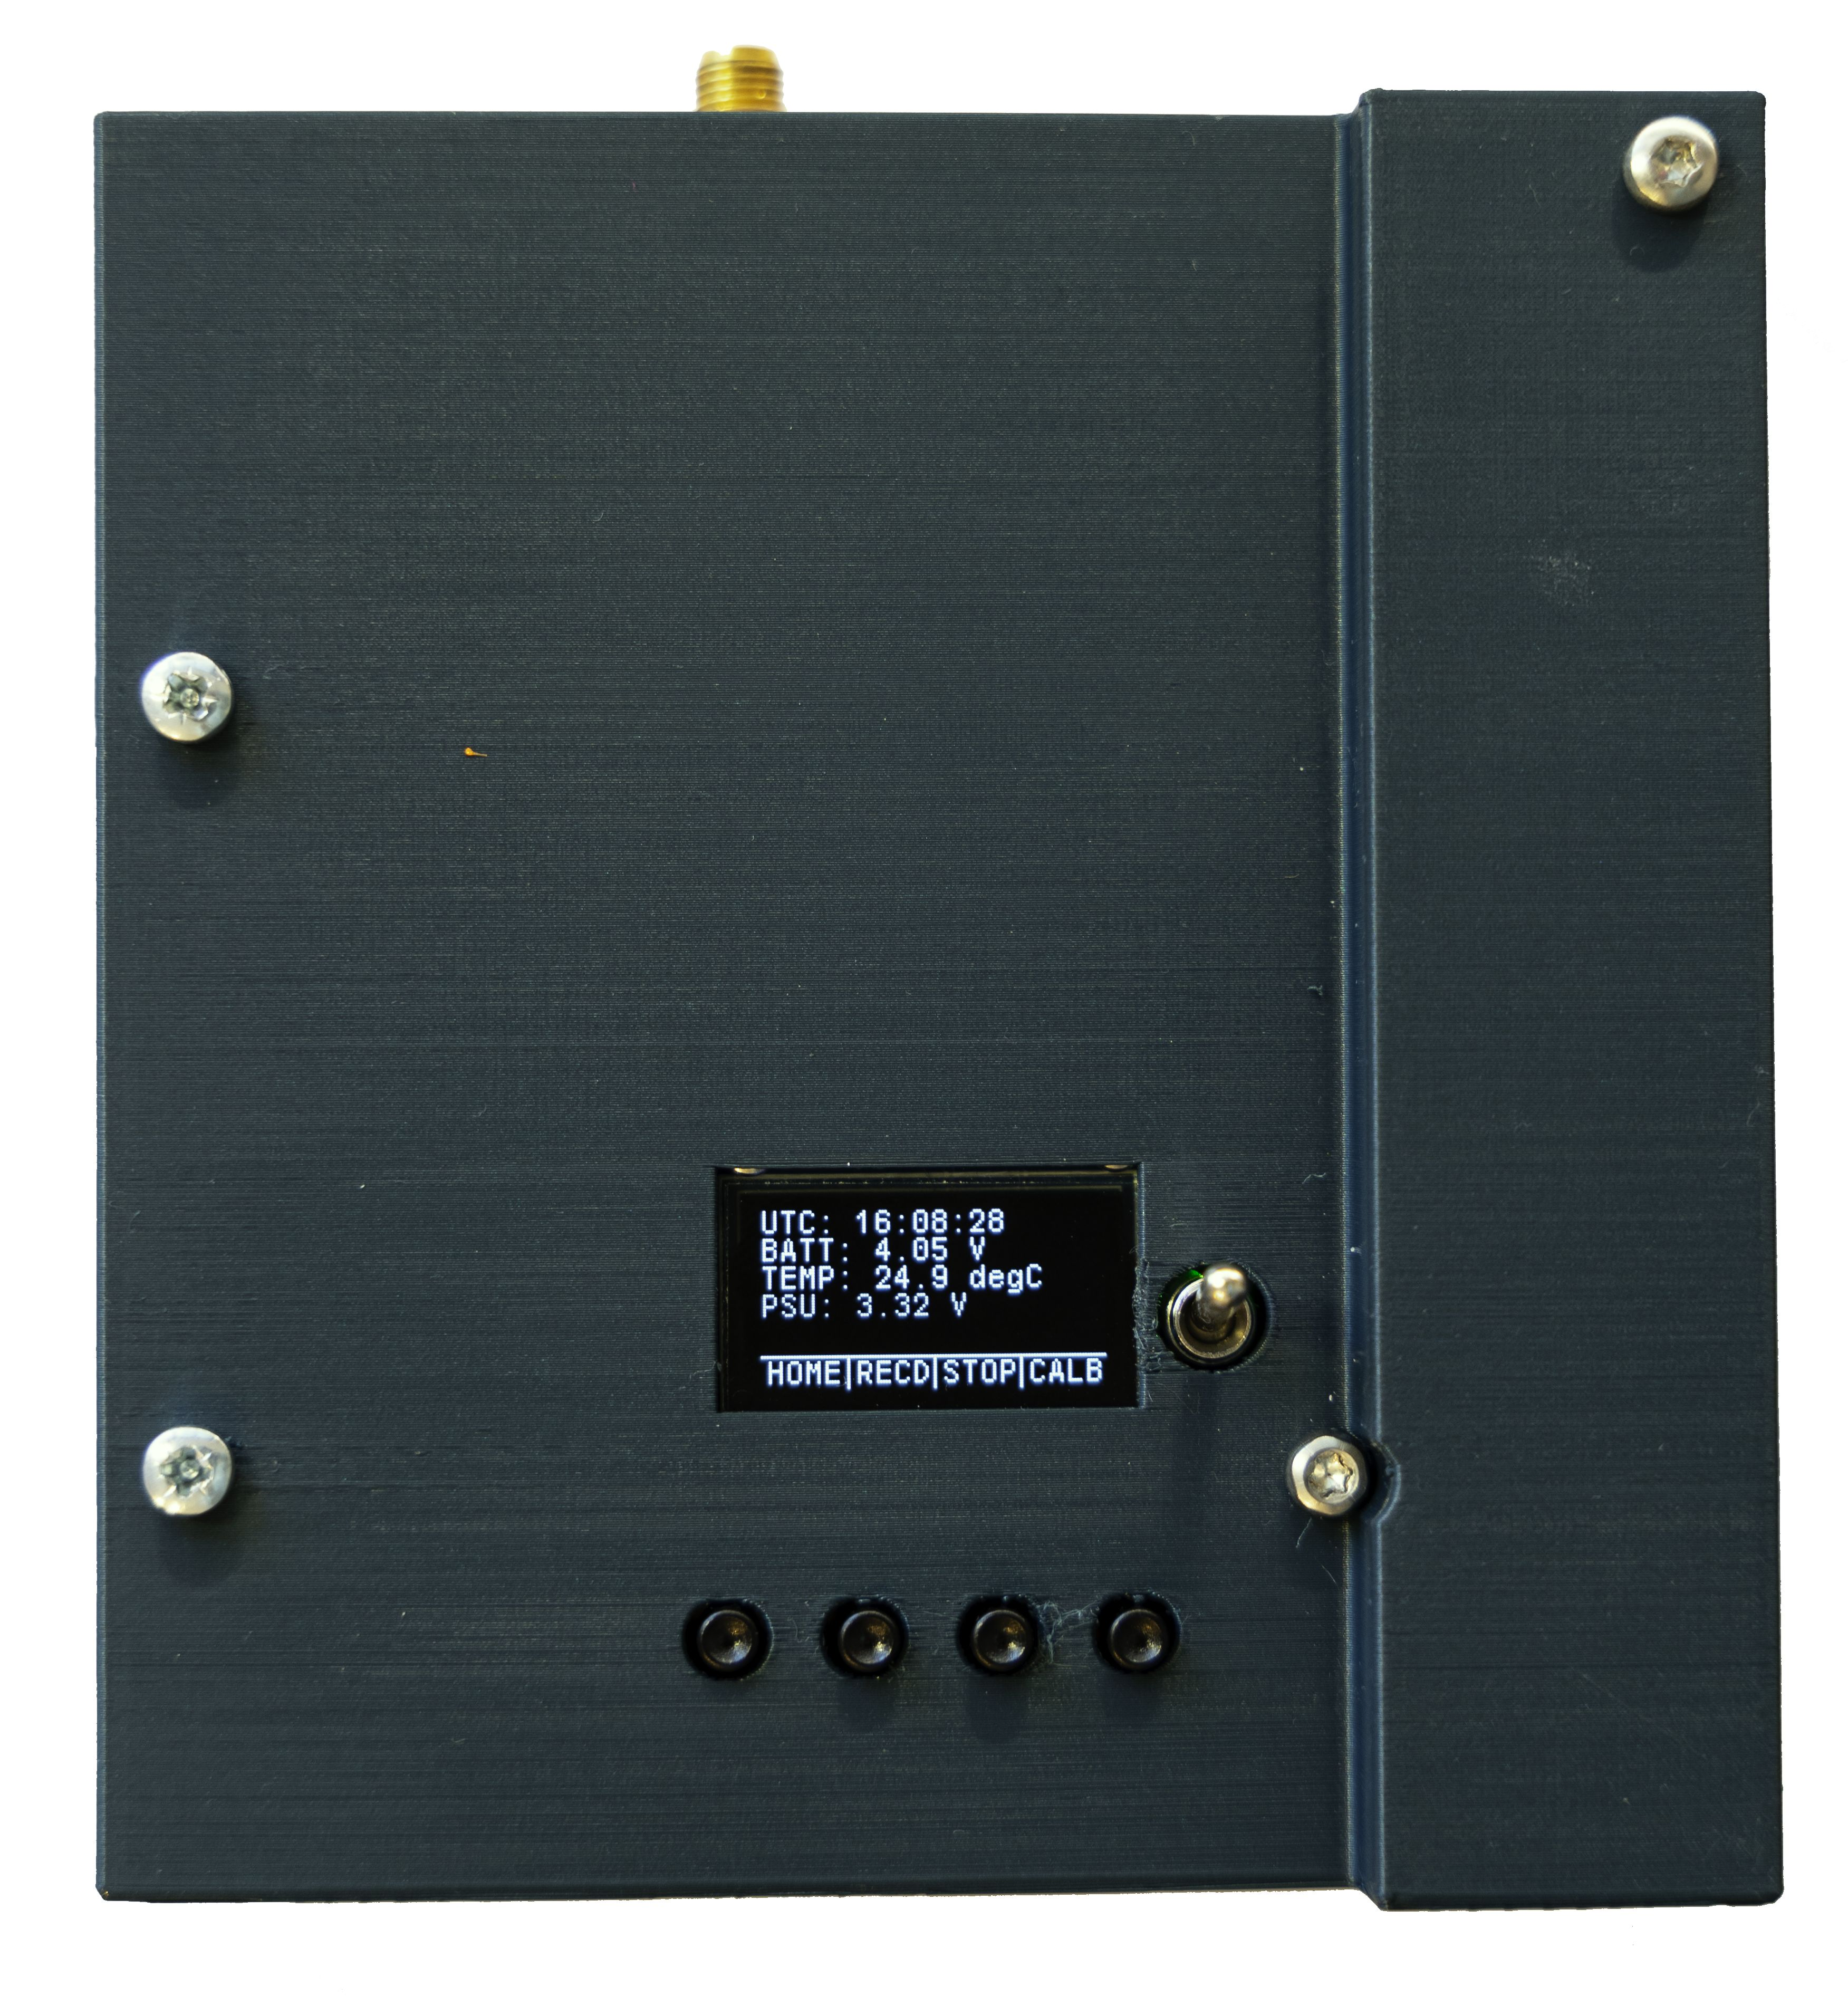
\includegraphics[width=\textwidth]{obrazky/ImunavFront}
         \caption{Hotová sestava.}
         
     \end{subfigure}
        \caption{Fotografie zařízení.}
        \label{fig:boxPhoto}
\end{figure}

\section{Ověření základních funkcí hardwaru jednotky}
Při prvním zapnutí desky byl k napájení použit laboratorní zdroj s proudovým omezením místo Li-Ion akumulátoru, aby v případě chyby v zapojení byla co nejvíce omezena šance poškození součástek. Zařízení při použití napájecího napětí 4 V odebíralo proud zhruba 198 mA, což je v tolerovaných mezích. Dále bylo zkontrolováno, zdali 3,3V snižující měnič, který napájí všechny citlivé komponenty, pracuje správně. Bylo změřeno napětí 3,313 V na jeho výstupu, je tedy v pořádku.

Jako další důležitý blok byla zkontrolována funkčnost S/R klopného obvodu, který poskytuje ochranu proti podvybití, popsanou v kapitole \ref{napajeni}. K tomuto byl vytvořen jednoduchý firmware procesoru, který průběžně měří napětí akumulátoru pomocí \ac{ADC} a v případě, že klesne pod úroveň 3,5 V přepne pin na vstupu KO do stavu logické jedničky. Tento stav byl simulován postupným snižováním výstupního napětí laboratorního zdroje. K vypnutí zařízení došlo při 3,54 V a ve vypnutém stavu zařízení odebíralo proud $ \SI{19,73}{\micro\ampere} $, což je spotřeba samotných klopných obvodů a \ac{RTC} zálohovacích registrů \ac{MCU} a \ac{GNSS} modulu. Při tomto napětí zbývá v akumulátoru zhruba 10 \% energie \cite{Cheruiyot2022914}, můžeme tedy vypočítat jak dlouho je možné ponechat zařízení softwarově vypnuté se sepnutým hlavním vypínačem, aniž by došlo k degradaci akumulátoru

\begin{equation}
t = \dfrac{C\cdot 0,1}{I}=\dfrac{2,9\cdot 0,1}{19,73 \cdot 10^{-6}}= \SI{1.68}{\roku} ,
\end{equation}
kde C je kapacita akumulátoru v ampérhodinách a I je proudový odběr vypnutého zařízení.

Při připojení zařízení ke zdroji pomocí \ac{USB} bylo napájení obnoveno, což je žádoucí. Také byla zkontrolována proudová spotřeba při nabíjení akumulátoru pomocí orientačního \ac{USB} měřicího přístroje TC66C, ta byla 751 mA v případě, že je zařízení zapnuté a akumulátor se nabíjí.

Další části zařízení jsou úzce vázány na software, jejich funkčnost byla tedy postupně testována při vývoji. Později byl odhalen drobný nedostatek hardwarového návrhu, a to v oblasti \ac{RTC} periferie hlavního procesoru. Ta slouží k udržení aktuálního času, který je možné synchronizovat například pomocí \ac{GNSS}. Z tohoto důvodu výrobce \ac{MCU} umožňuje napájet periferii pomocí separátního pinu \emph{VBAT} který je využíván při vypnutém hlavním napájení a má velice malý proudový odběr, jehož zdrojem je lineární napěťový regulátor s malým klidovým proudem připojeným přímo k akumulátoru. Vzhledem k tomu, že tato funkcionalita není pro aplikaci inerciální navigace klíčová a jedná se pouze o možnost zvýšení pohodlí uživatele, tak nebyly kladeny vysoké nároky na její přesnost, proto nebyl zapojen externí nízkofrekvenční krystalový oscilátor \emph{LSE} s domněním, že bude postačovat pouze interní oscilátor \emph{LSI RC}. Ukázalo se ovšem, že z napájecí domény \emph{VBAT} je poskytováno napájení pouze externímu nízkofrekvenčnímu oscilátoru, nikoliv internímu \cite{csdGtKJDMSdbwJ9r}. Z tohoto důvodu byl dodatečně přidán 32,768kHz krystal, společně se zatěžovacími kondenzátory (viz. obrázek \ref{fig:RTCcrystal}), který byl po otestování připevněn lepidlem.


\begin{figure}[h]
    \centering
    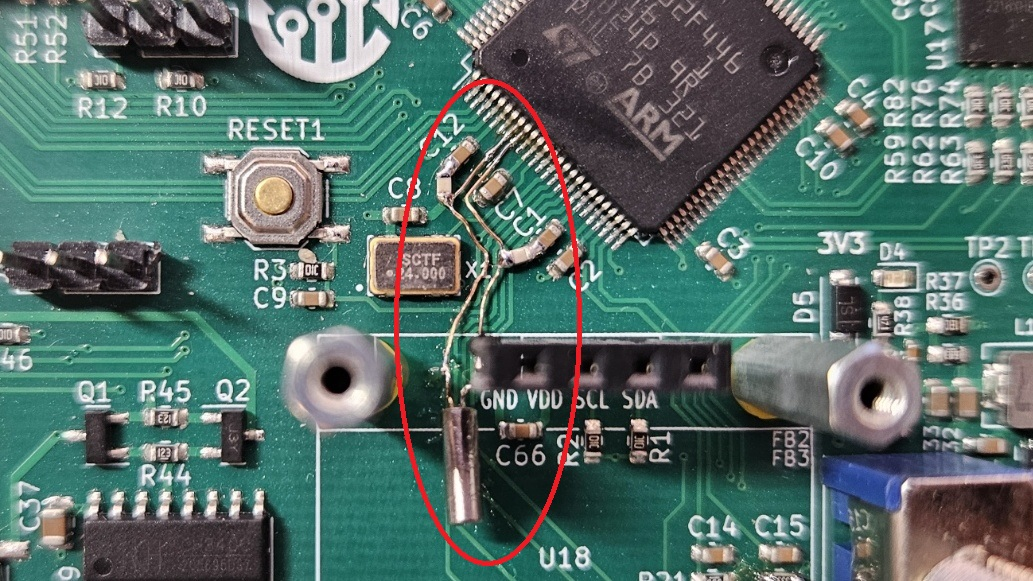
\includegraphics[width=0.8\textwidth]{obrazky/RTCcrystal}
    \caption{Dodatečná oprava RTC oscilátoru.}
    \label{fig:RTCcrystal}
\end{figure}








\chapter*{Závěr}
\phantomsection
\addcontentsline{toc}{chapter}{Závěr}
V rámci semestrální práce jsme popsali kinematiku pohybu a nakládání s veličinami změřenými IMU pro potřeby výpočtu polohy. Také jsme definovali několik vztažných soustav a postupy pro převod mezi nimi. Je rozebráno tíhové pole Země, gravitační modely a jejich význam v inerciální navigaci.

Byl popsán funkční princip IMU a společně s GNSS modulem s možností inerciální navigace byly vyzkoušeny a otestovány pomocí běžně dostupných vývojových stavebnic.

Práce se také věnuje návrhu obvodového zapojení inerciální jednotky, definováním minimálních požadavků na hlavní MCU tak, abychom nebyli v budoucnu omezeni některým z rozhodnutí při návrhu hardwaru. Inerciální jednotka byla osazena i jinými senzory než gyroskopy a akcelerometry pro možnou senzorickou fúzi v bakalářské práci.

V neposlední řadě se také věnujeme návrhu samotné DPS v programu KiCad, jejíž výkresy a schéma jsou v příloze. Deska je v čase psaní této práce buď vyráběna, nebo již čeká na doručení.

%%% Vložení souboru 'text/literatura' se seznamem zdrojů
%\begin{thebibliography}{13}

\bibitem{mGnys3WmOkWuaQHN}
TEXAS INSTRUMENTS. \textit{TPS6282x: 5.5-V, 1-A, 2-A, 3-A Step-Down Converter Family with 1\% Accuracy}. Online katalogový list. C. 2019. Dostupné z: \url{https://www.ti.com/lit/gpn/tps62823}. [cit. 2023-12-21].
\bibitem{F5eZCtr2LLRsr9NT}
TEXAS INSTRUMENTS. \textit{BQ2407x: Standalone 1-Cell 1.5-A Linear Battery Chargers with Power Path}. Online katalogový list. N. 2021. Dostupné z: \url{https://www.ti.com/lit/gpn/bq24075}. [cit. 2023-12-21].
\bibitem{zJ7x5ye8Y5eJn1E2}
ESPRESSIF SYSTEMS. \textit{ESP32C3MINI1: Smallsized 2.4 GHz WiFi (802.11 b/g/n) and Bluetooth® 5 module}. Online katalogový list. 2022. Dostupné z: \url{https://www.espressif.com/sites/default/files/documentation/esp32-c3-mini-1\_datasheet\_en.pdf}. [cit. 2023-12-21].
\bibitem{Kraewinkel2020}
KRÄWINKEL, R.W. \textit{The effect of writing and transmitting SD card data on the consistency of SD card write performance}. Online, bakalářská. Enschede, Holandsko: University of Twente, 2020. Dostupné z: \url{http://essay.utwente.nl/82256/1/Krawinkel\_BA\_EEMCS.pdf}. [cit. 2023-12-17].
\bibitem{CgaRYSTpwKhEZZr7}
XTX TECHNOLOGY LIMITED. \textit{XT25F256BWSIGT: Quad IO Serial NOR Flash Datasheet}. Online katalogový list. 2020. Dostupné z: \url{http://www.xtxtech.com/download/?AId=287}. [cit. 2023-12-17].
\bibitem{DLQg9bT6V1GWKhxh}
U-BLOX. \textit{NEO-M8U: u-blox M8 untethered dead reckoning module including 3D inertial sensors}. Online katalogový list. R13. 2022. Dostupné z: \url{https://content.u-blox.com/sites/default/files/NEO-M8U\_DataSheet\_UBX-15015679.pdf}. [cit. 2023-12-17].
\bibitem{Tkhorenko2018}
TKHORENKO, M. Yu.; PAVLOV, B. V.; KARSHAKOV, E. V. a VOLKOVITSKY, A. K. On integration of a strapdown inertial navigation system with modern magnetic sensors. Online. In: \textit{2018 25th Saint Petersburg International Conference on Integrated Navigation Systems (ICINS)}. IEEE, 2018, s.~1-4. ISBN 978-5-91995-057-8. Dostupné z: \url{https://doi.org/10.23919/ICINS.2018.8405845}. [cit. 2023-12-17].
\bibitem{Wei2022}
WEI, Y. a LI, Y. IMPACT OF SENSOR DATA SAMPLING RATE IN GNSS/INS INTEGRATED NAVIGATION WITH VARIOUS SENSOR GRADES. Online. \textit{The International Archives of the Photogrammetry, Remote Sensing and Spatial Information Sciences}. 2022, roč. XLVI-3/W1-2022, s.~205-211. ISSN 2194-9034. Dostupné z: \url{https://doi.org/10.5194/isprs-archives-XLVI-3-W1-2022-205-2022}. [cit. 2023-12-16].
\bibitem{euxR3Yh5ol4JWNAi}
TDK INVENSENSE. \textit{MPU6050: Product specification}. Online katalogový list. 3.4. 2013. Dostupné z: \url{https://invensense.tdk.com/wp-content/uploads/2015/02/MPU-6000-Datasheet1.pdf}. [cit. 2023-12-12].
\bibitem{UZFqHmQU7ZzI3OLB}
ANALOG DEVICES. \textit{ADIS16505: Precision, Miniature MEMS IMU}. Online katalogový list. C. 2020. Dostupné z: \url{https://www.analog.com/media/en/technical-documentation/data-sheets/adis16505.pdf}. [cit. 2023-12-12].
\bibitem{RD5DwZcremhT6bgp}
ST MICROELECTRONICS. \textit{LSM303AGR: Ultracompact high-performance eCompass module}. Online katalogový list. 11. 2022. Dostupné z: \url{https://www.st.com/resource/en/datasheet/lsm303agr.pdf}. [cit. 2023-12-12].
\bibitem{csdGtKJDMSdbwJ9r}
ST MICROELECTRONICS. \textit{STM32F446xC/E: Arm® Cortex®-M4 32-bit MCU+FPU, 225 DMIPS, up to 512 KB Flash/128+4 KB RAM, USB OTG HS/FS, seventeen TIMs, three ADCs and twenty communication interfaces}. Online katalogový list. 10. 2021. Dostupné z: \url{https://www.st.com/resource/en/datasheet/stm32f446ve.pdf}. [cit. 2023-12-14].
\bibitem{Blocher2021322}
BLOCHER, Lukas; MAYER, Wolfram; ARENA, Marco; RADOVIC, Dusan; HILLER, Tobias et al. Purely Inertial Navigation with a Low-Cost MEMS Sensor Array. Online. In: \textit{2021 IEEE International Symposium on Inertial Sensors and Systems (INERTIAL)}. IEEE, 2021, s.~1-4. ISBN 978-1-7281-5099-4. Dostupné z: \url{https://doi.org/10.1109/INERTIAL51137.2021.9430468}. [cit. 2023-12-09].

\end{thebibliography}
\begin{thebibliography}{99}

\bibitem{Tittertonc2004}TITTERTON, D. H. a WESTON, J. L. \textit{Strapdown inertial navigation technology}. Second edition. Progress in astronautics and aeronautics, 207. Reston, VA: American Institute of Aeronautics and Astronautics, c2004. ISBN 1-56347-693-2.

\bibitem{Grewal2013}GREWAL, Mohinder S.; ANDREWS, Angus P. a BARTONE, Chris. \textit{Global navigation satellite systems, inertial navigation, and integration}. Third edition. Hoboken, New Jersey: John Wiley, 2013. ISBN 978-1-118-44700-0.

\bibitem{Polak2018}POLÁK, Luboš. \textit{Navigační jednotka s modifikovanou soustavou akcelerometrů}. Online, Bakalářská práce. Praha: České vysoké učení technické v Praze, Fakulta elektrotechnická, 2018. Dostupné z: \url{http://hdl.handle.net/10467/74430}. [cit. 2023-12-25].

\bibitem{Pekarek2020}PEKÁREK, David. \textit{Přesné meření vlastní trajektorie vozidla}. Online, Bakalářská práce. Praha: České vysoké učení technické v Praze, Fakulta elektrotechnická, 2020. Dostupné z: \url{http://hdl.handle.net/10467/90221}. [cit. 2023-12-25].

\bibitem{Halliday2000}HALLIDAY, David; RESNICK, Robert a WALKER, Jearl. \textit{Fyzika: vysokoškolská učebnice obecné fyziky}. Překlady vysokoškolských učebnic. Brno: VUTIUM, 2000. ISBN 80-214-1869-9.

\bibitem{Pavlis2012}PAVLIS, Nikolaos K.; HOLMES, Simon A.; KENYON, Steve C. a FACTOR, John K. The development and evaluation of the Earth Gravitational Model 2008 (EGM2008). Online. \textit{Journal of Geophysical Research: Solid Earth}. 2012, roč. 117, č. B4, s.~1-38. ISSN 0148-0227. Dostupné z: \url{https://doi.org/10.1029/2011JB008916}. [cit. 2023-12-26].

\bibitem{Bezdek2013}BEZDĚK, Aleš a SEBERA, Josef. Matlab script for 3D visualizing geodata on a rotating globe. Online. \textit{Computers and Geosciences}. 2013, roč. 56, s.~127-130. ISSN 00983004. Dostupné z: \url{https://doi.org/10.1016/j.cageo.2013.03.007}. [cit. 2023-12-26].

\bibitem{Dadafshar2014}DADAFSHAR, Majid. \textit{APPLICATION NOTE 5830: ACCELEROMETER AND GYROSCOPES SENSORS: OPERATION, SENSING, AND APPLICATIONS}. Online aplikační poznámka. 2014. Dostupné z: \url{https://pdfserv.maximintegrated.com/en/an/AN5830.pdf}. [cit. 2023-12-27].

\bibitem{cCumN04KaPNjERaF}MNX. \textit{What is Mems Technology?} Online. MEMS and Nanotechnology Exchange. Dostupné z: \url{https://www.mems-exchange.org/MEMS/what-is.html}. [cit. 2023-12-27].

\bibitem{Blocher2021322}BLOCHER, Lukas; MAYER, Wolfram; ARENA, Marco; RADOVIC, Dusan; HILLER, Tobias et al. Purely Inertial Navigation with a Low-Cost MEMS Sensor Array. Online. In: \textit{2021 IEEE International Symposium on Inertial Sensors and Systems (INERTIAL)}. IEEE, 2021, s.~1-4. ISBN 978-1-7281-5099-4. Dostupné z: \url{https://doi.org/10.1109/INERTIAL51137.2021.9430468}. [cit. 2023-12-09].

\bibitem{euxR3Yh5ol4JWNAi}TDK INVENSENSE. \textit{MPU6050: Product specification}. Online katalogový list. 3.4. 2013. Dostupné z: \url{https://invensense.tdk.com/wp-content/uploads/2015/02/MPU-6000-Datasheet1.pdf}. [cit. 2023-12-12].

\bibitem{Wei2022}WEI, Y. a LI, Y. IMPACT OF SENSOR DATA SAMPLING RATE IN GNSS/INS INTEGRATED NAVIGATION WITH VARIOUS SENSOR GRADES. Online. \textit{The International Archives of the Photogrammetry, Remote Sensing and Spatial Information Sciences}. 2022, roč. XLVI-3/W1-2022, s.~205-211. ISSN 2194-9034. Dostupné z: \url{https://doi.org/10.5194/isprs-archives-XLVI-3-W1-2022-205-2022}. [cit. 2023-12-16].

\bibitem{UZFqHmQU7ZzI3OLB}ANALOG DEVICES. \textit{ADIS16505: Precision, Miniature MEMS IMU}. Online katalogový list. C. 2020. Dostupné z: \url{https://www.analog.com/media/en/technical-documentation/data-sheets/adis16505.pdf}. [cit. 2023-12-12].

\bibitem{Tkhorenko2018}TKHORENKO, M. Yu.; PAVLOV, B. V.; KARSHAKOV, E. V. a VOLKOVITSKY, A. K. On integration of a strapdown inertial navigation system with modern magnetic sensors. Online. In: \textit{2018 25th Saint Petersburg International Conference on Integrated Navigation Systems (ICINS)}. IEEE, 2018, s.~1-4. ISBN 978-5-91995-057-8. Dostupné z: \url{https://doi.org/10.23919/ICINS.2018.8405845}. [cit. 2023-12-17].

\bibitem{RD5DwZcremhT6bgp}ST MICROELECTRONICS. \textit{LSM303AGR: Ultracompact high-performance eCompass module}. Online katalogový list. 11. 2022. Dostupné z: \url{https://www.st.com/resource/en/datasheet/lsm303agr.pdf}. [cit. 2023-12-12].

\bibitem{DLQg9bT6V1GWKhxh}U-BLOX. \textit{NEO-M8U: u-blox M8 untethered dead reckoning module including 3D inertial sensors}. Online katalogový list. R13. 2022. Dostupné z: \url{https://content.u-blox.com/sites/default/files/NEO-M8U\_DataSheet\_UBX-15015679.pdf}. [cit. 2023-12-17].

\bibitem{CgaRYSTpwKhEZZr7}XTX TECHNOLOGY LIMITED. \textit{XT25F256BWSIGT: Quad IO Serial NOR Flash Datasheet}. Online katalogový list. 2020. Dostupné z: \url{http://www.xtxtech.com/download/?AId=287}. [cit. 2023-12-17].

\bibitem{Kraewinkel2020}KRÄWINKEL, R.W. \textit{The effect of writing and transmitting SD card data on the consistency of SD card write performance}. Online, bakalářská. Enschede, Holandsko: University of Twente, 2020. Dostupné z: \url{http://essay.utwente.nl/82256/1/Krawinkel\_BA\_EEMCS.pdf}. [cit. 2023-12-17].

\bibitem{F5eZCtr2LLRsr9NT}TEXAS INSTRUMENTS. \textit{BQ2407x: Standalone 1-Cell 1.5-A Linear Battery Chargers with Power Path}. Online katalogový list. N. 2021. Dostupné z: \url{https://www.ti.com/lit/gpn/bq24075}. [cit. 2023-12-21].

\bibitem{mGnys3WmOkWuaQHN}TEXAS INSTRUMENTS. \textit{TPS6282x: 5.5-V, 1-A, 2-A, 3-A Step-Down Converter Family with 1\% Accuracy}. Online katalogový list. C. 2019. Dostupné z: \url{https://www.ti.com/lit/gpn/tps62823}. [cit. 2023-12-21].

\bibitem{csdGtKJDMSdbwJ9r}\textit{STM32F446xC/E: Arm® Cortex®-M4 32-bit MCU+FPU, 225 DMIPS, up to 512 KB Flash/128+4 KB RAM, USB OTG HS/FS, seventeen TIMs, three ADCs and twenty communication interfaces}. Online katalogový list. 10. 2021. Dostupné z: \url{https://www.st.com/resource/en/datasheet/stm32f446ve.pdf}. [cit. 2023-12-14].

\bibitem{zJ7x5ye8Y5eJn1E2}ESPRESSIF SYSTEMS. \textit{ESP32C3MINI1: Smallsized 2.4 GHz WiFi (802.11 b/g/n) and Bluetooth® 5 module}. Online katalogový list. 2022. Dostupné z: \url{https://www.espressif.com/sites/default/files/documentation/esp32-c3-mini-1\_datasheet\_en.pdf}. [cit. 2023-12-21].

\bibitem{Cheruiyot2022914}CHERUIYOT, Fabian; SEGERA, Davies a OSORIO DE LA ROSA, Edith. A Master-Slave Salp Swarm Algorithm Optimizer for Hybrid Energy Storage System Control Strategy in Electric Vehicles. Online. \textit{Journal of Energy}. 2022, roč. 2022, s.~1-20. ISSN 2314-615X. Dostupné z: \url{https://doi.org/10.1155/2022/1648433}. [cit. 2024-05-13].

\bibitem{V2Tf5wsrbWcbQdoW}ST MICROELECTRONICS. \textit{UM2609: STM32CubeIDE user guide}. Online uživatelský návod. 11. 2024. Dostupné z: \url{https://www.st.com/resource/en/user\_manual/um2609-stm32cubeide-user-guide-stmicroelectronics.pdf}. [cit. 2024-05-14].

\bibitem{Zhu2011}ZHU, Ming-Yuan. \textit{Understanding FreeRTOS: A Requirement Analysis}. Online. ResearchGate, 2011. Dostupné z: \url{https://doi.org/10.13140/RG.2.2.12419.09767}. [cit. 2024-05-14].

\bibitem{SimpleMethod2021}SIMPLEMETHOD. \textit{STM32 library with DMA support for u-blox devices supporting Global Navigation Satellite Systems and UBX standard}. Online. Nenalezený vydavatel. 2021. Dostupné z: \url{https://github.com/SimpleMethod/STM32-GNSS}. [cit. 2024-05-16].

\bibitem{Alekseev2024}ALEKSEEV, Aleksander. \textit{STM32 library for working with OLEDs based on SSD1306}. Online. GitHub. 2024. Dostupné z: \url{https://github.com/afiskon/stm32-ssd1306}. [cit. 2024-05-16].


\bibitem{eUM5mr8dMf0LyseX}ST MICROELECTRONICS. \textit{AN4508: Parameters and calibration of a low-g 3-axis accelerometer}. Online aplikační poznámka. 2014. Dostupné z: \url{https://www.st.com/resource/en/application\_note/an4508-parameters-and-calibration-of-a-lowg-3axis-accelerometer-stmicroelectronics.pdf}. [cit. 2023-05-20].


\bibitem{6yeG6wAI1hTfmXJK}FREESCALE SEMICONDUCTOR. \textit{AN4399: High-Precision Calibration of a Three-Axis Accelerometer}. Online aplikační poznámka. 2. 2015. Dostupné z: \url{https://www.nxp.com/docs/en/application-note/AN4399.pdf}. [cit. 2023-05-20].

\bibitem{M7nvHLyk8N0V3ub2}MATHWORKS. \textit{Navigation Toolbox User's Guide}. Online. 24.1. 2024. Dostupné z: \url{https://www.mathworks.com/help/pdf\_doc/nav/nav\_ug.pdf}. [cit. 2024-05-22].

\end{thebibliography}

%%% Vložení souboru 'text/zkratky' se seznam použitých symbolů, veličin a zkratek
\cleardoublepage
\chapter*{\listofabbrevname}
\phantomsection
\addcontentsline{toc}{chapter}{\listofabbrevname}

\begin{acronym}[KolikMista]
\acro{DoF}{Degrees of Freedom - stupně volnosti}
\acro{IMU}{Inertial Measurement Unit - měřicí inerciální jednotka}
\acro{OLED}{}
\acro{MCU}{}
\acro{GPS}{}
\acro{IMU}{}
\acro{MEMS}{}
\acro{I2C}{}
\acro{FIFO}{}
\acro{BGA}{}
\acro{DPS}{}
\acro{RAM}{}
\acro{ADC}{}

	%%% esymfvz

\end{acronym}

%\acro{ADC}{Analog to Digital Convertor - analogově-digitální převodník}
\acro{BGA}{Ball Grid Array - pouzdro matice kuliček}
\acro{CAD}{Computer-Aided Design - počítačem podporované projektování}
\acro{CSV}{Comma Separated Value - čárkou oddělené hodnoty}
\acro{DMA}{Direct Memory Acces - přímý přístup k paměti}
\acro{DoF}{Degrees of Freedom - stupně volnosti}
\acro{DPS}{Deska Plošných Spojů}
\acro{EGM}{Earth Gravitational Model - gravitační model Země}
\acro{FIFO}{First In First Out - první dovnitř, první ven}
\acro{GNSS}{Global navigation satellite system - globální družicový polohový systém}
\acro{GPIO}{General Purpose Input/Output - univerzální vstupní/výstupní pin}
\acro{GPS}{Global Positioning System - globální polohový systém}
\acro{GUI}{Graphical User Interface - grafické uživatelské rozhraní}
\acro{HAL}{Hardware Abstraction Layer - vrstva abstrakce hardwaru}
\acro{I2C}{Inter-Integrated Circuit - mezi obvodová komunikace}
\acro{IDE}{Integrated Developement Enviroment - vývojové prostředí}
\acro{IMU}{Inertial Measurement Unit - měřicí inerciální jednotka}
\acro{IMU}{Inertial Measurement Unit - inerciální měřicí jednotka}
\acro{MCU}{Microcontroller Unit - mikrokontrolér}
\acro{MEMS}{Micro-ElectroMechanical Systems - mikro-elektromechanické systémy}
\acro{MSC}{Mass Storage Class - třída paměťového média}
\acro{NED}{North East Down - sever východ dolů}
\acro{NGA}{National Geospatial-Intelligence Agency - americká geoprostorová agentura}
\acro{NMEA}{National Marine Electronics Association - americká organizace námořní elektroniky}
\acro{OLED}{Organic Light-Emitting Diode - orgranický LED}
\acro{PID}{Product ID - identifikace produktu}
\acro{RAM}{Random Access Memory - paměť pro náhodný přístup}
\acro{RTC}{Real Time Clock - obvod reálného času}
\acro{RTOS}{Real Time Operating System - Operační systém reálného času}
\acro{SMA}{SubMiniature~version A - subminiaturní verze A}
\acro{SPI}{Serial Peripheral Interface - sériové periferní rozhraní}
\acro{UART}{Universal Asynchronous Receiver-Transmitter - univerzální asynchronní přijímač-vysílač}
\acro{UBX}{UBloX message - zpráva formátu UBLOX}
\acro{USB}{Universal Serial Bus - univerzální sériová sběrnice}
\acro{VID}{Vendor ID - identifikace výrobce}

%%% Začátek příloh
\appendix

%%% Vysázení seznamu příloh
% (vynechejte, pokud máte dvě nebo méně příloh)
\listofappendices

%%% Vložení souboru 'text/prilohy' s přílohami
% Obvykle je přítomen alespoň popis co najdeme na přiloženém médiu

\chapter{Obsah elektronické přílohy}

\dirtree{%
 .1 .
 .2 Firmware.
 .3 IMUnav\_STM\_F00.
 .4 Core.
 .5 AccelCalSolver.
 .6 \dots.
 .5 Inc.
 .6 \dots.
 .5 Src.
 .6 \dots.
 .4 Debug.
 .5 \dots.
 .4 Drivers.
 .5 \dots.
 .4 FATFS.
 .5 \dots.
 .4 Middlewares.
 .5 \dots.
 .4 Release.
 .5 \dots.
 .4 USB\_DEVICE.
 .5 \dots.
 .4 IMUnav\_STM\_F00 Debug.launch.
 .4 IMUnav\_STM\_F00.ioc.
 .4 STM32F446VETX\_FLASH.ld.
 .4 STM32F446VETX\_RAM.ld.
 .2 Hardware.
 .3 IMUnav-library.
 .4 \dots.
 .3 IMUnav\_H00.
 .4 bom.
 .5 ibom.html.
 .4 production.
 .5 \dots.
 .4 ESP32.kicad\_sch.
 .4 GPS.kicad\_sch.
 .4 IMU.kicad\_sch.
 .4 IMU.kicad\_sch-bak.
 .4 IMUnav\_H00.kicad\_dru.
 .4 IMUnav\_H00.kicad\_pcb.
 .4 IMUnav\_H00.kicad\_prl.
 .4 IMUnav\_H00.kicad\_pro.
 .4 IMUnav\_H00.kicad\_sch.
 .4 IMUnav\_H00.kicad\_sch-bak.
 .4 IMUnav\_H00.step.
 .4 Memory.kicad\_sch.
 .4 USB+Power.kicad\_sch.
 .4 User.kicad\_sch.
 .4 fp-info-cache.
 .4 fp-lib-table.
 .4 sym-lib-table.
 .2 Software.
 .3 Matlab.
 .4 C generator.
 .5 codegen.
 .6 lib.
 .7 \dots.
 .6 mex.
 .7 \dots.
 .5 AccelCalSolver.m.
 .5 AccelCalSolver.prj.
 .5 accelCalibration.m.
 .5 gravityFun.m.
 .4 IMUonlyNavigation.m.
 .4 chuzePoByte.csv.
 .4 chuzeVenkuCALB.csv.
 .4 ctverecChuze.csv.
 .4 ctverecChuze2.csv.
 .4 ctverecChuze3CALB.csv.
 .4 ctverecRychlaChuze.csv.
 .4 imuAndGnssInsfilterMARG.m.
 .4 koleckoKolemFEKTUCALB.csv.
 .4 tiltedStationary.csv.
 .3 Python.
 .4 IMUDATA.BIN.
 .4 binDecoder.py.
}

\chapter{Schéma zapojení inerciální jednotky} \label{schemaApp}
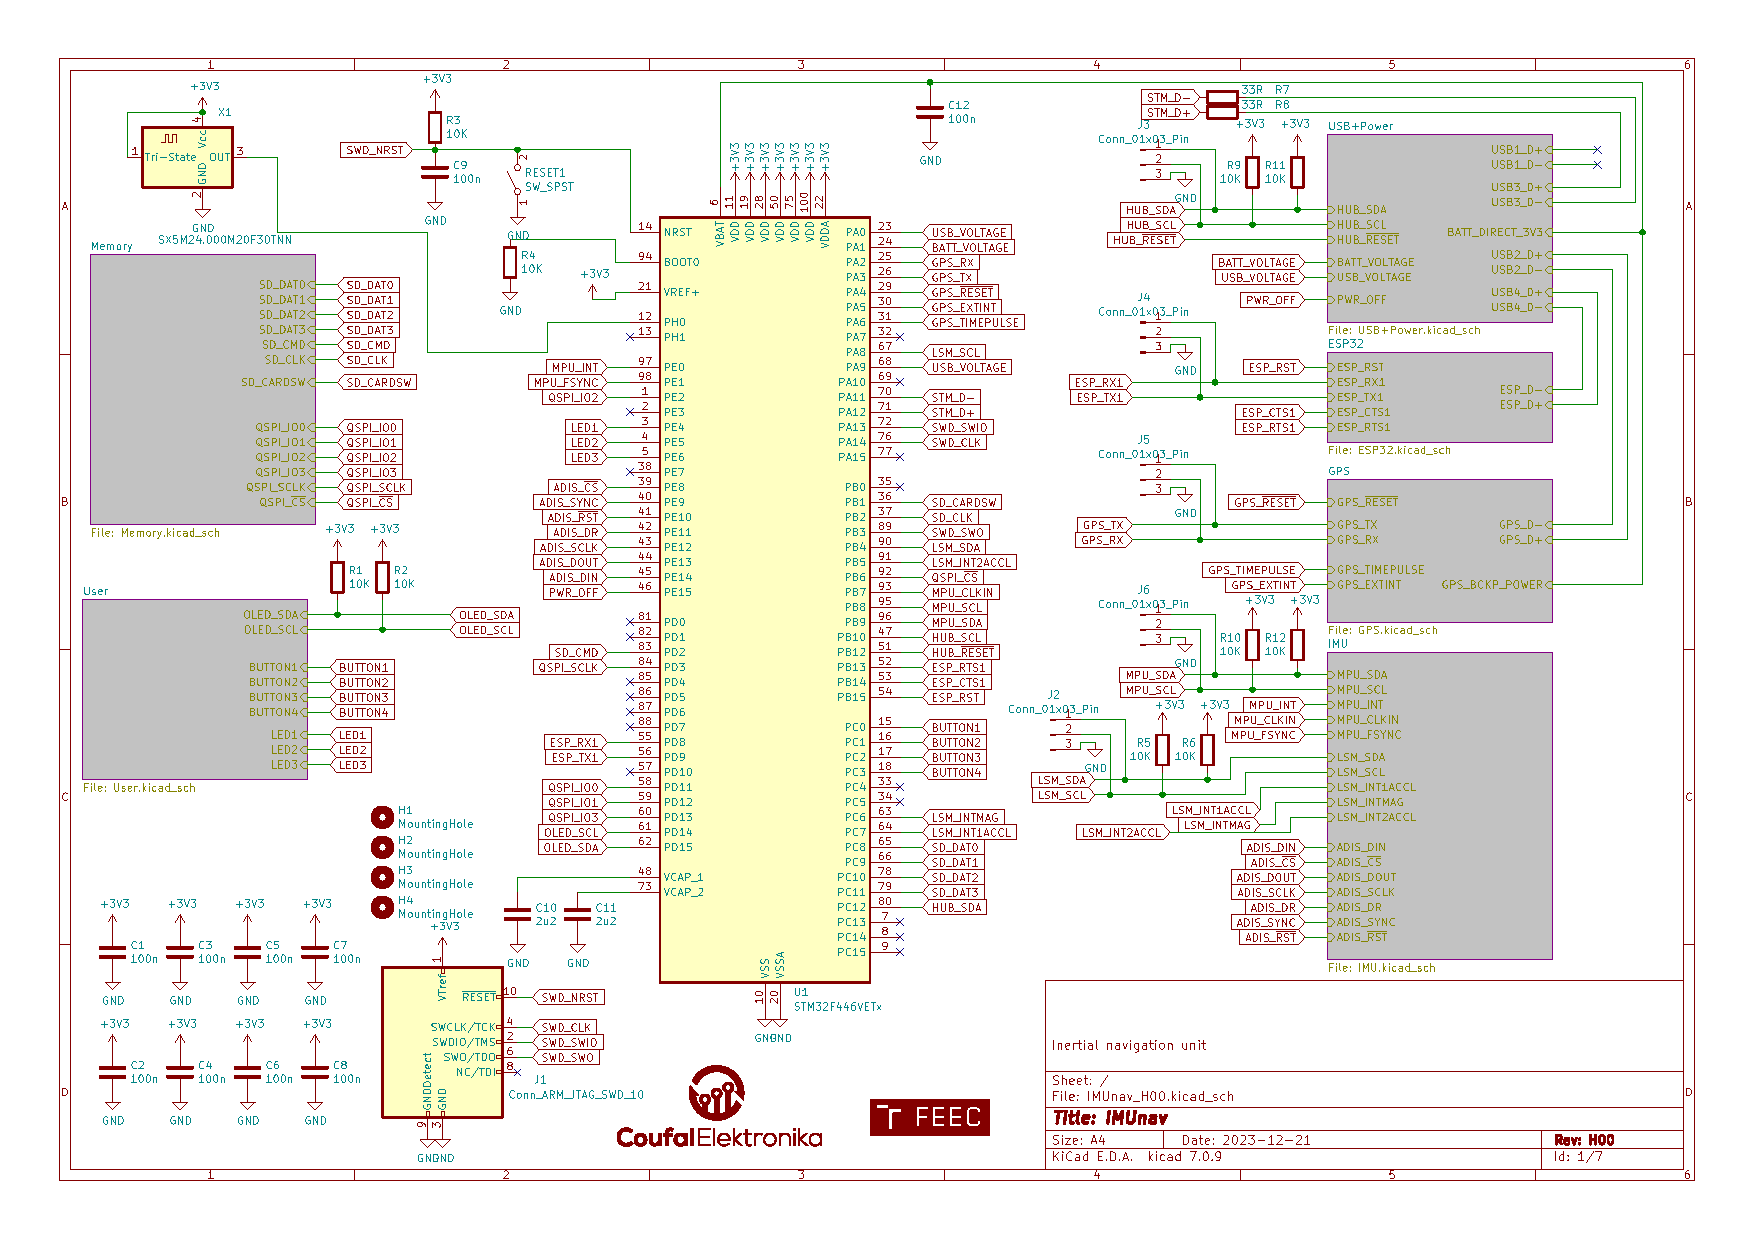
\includegraphics[angle=90, page=1, width=\textwidth]{KiCad/schematic.pdf}

\includegraphics[angle=90, page=2, width=\textwidth]{KiCad/schematic.pdf}

\includegraphics[angle=90, page=3, width=\textwidth]{KiCad/schematic.pdf}

\includegraphics[angle=90, page=4, width=\textwidth]{KiCad/schematic.pdf}

\includegraphics[angle=90, page=5, width=\textwidth]{KiCad/schematic.pdf}

\includegraphics[angle=90, page=6, width=\textwidth]{KiCad/schematic.pdf}

\includegraphics[angle=90, page=7, width=\textwidth]{KiCad/schematic.pdf}

\chapter{Výkres DPS}
\section{Pohled osazení součástek} \label{placementApp}
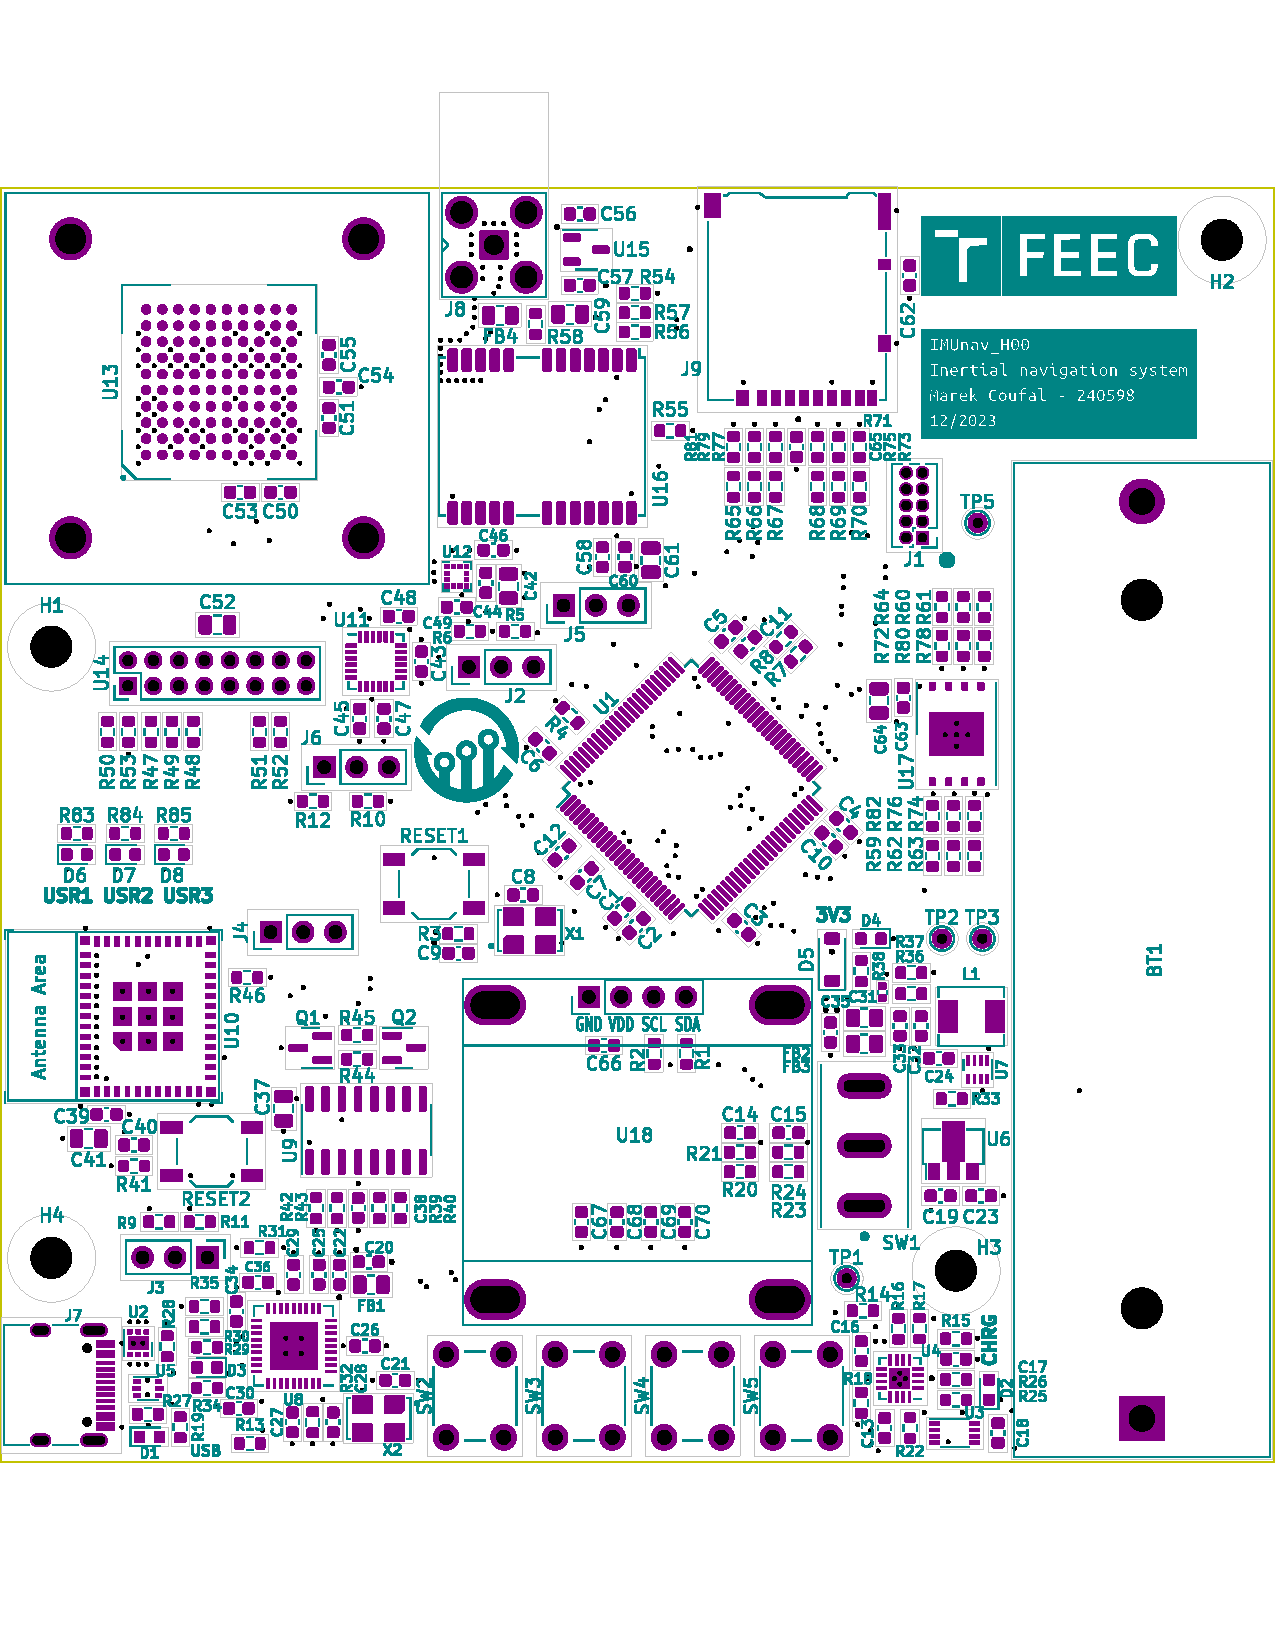
\includegraphics[width=\textwidth]{KiCad/boardTopParts}

\section{Vrchní vrstva mědi DPS} \label{TopApp}
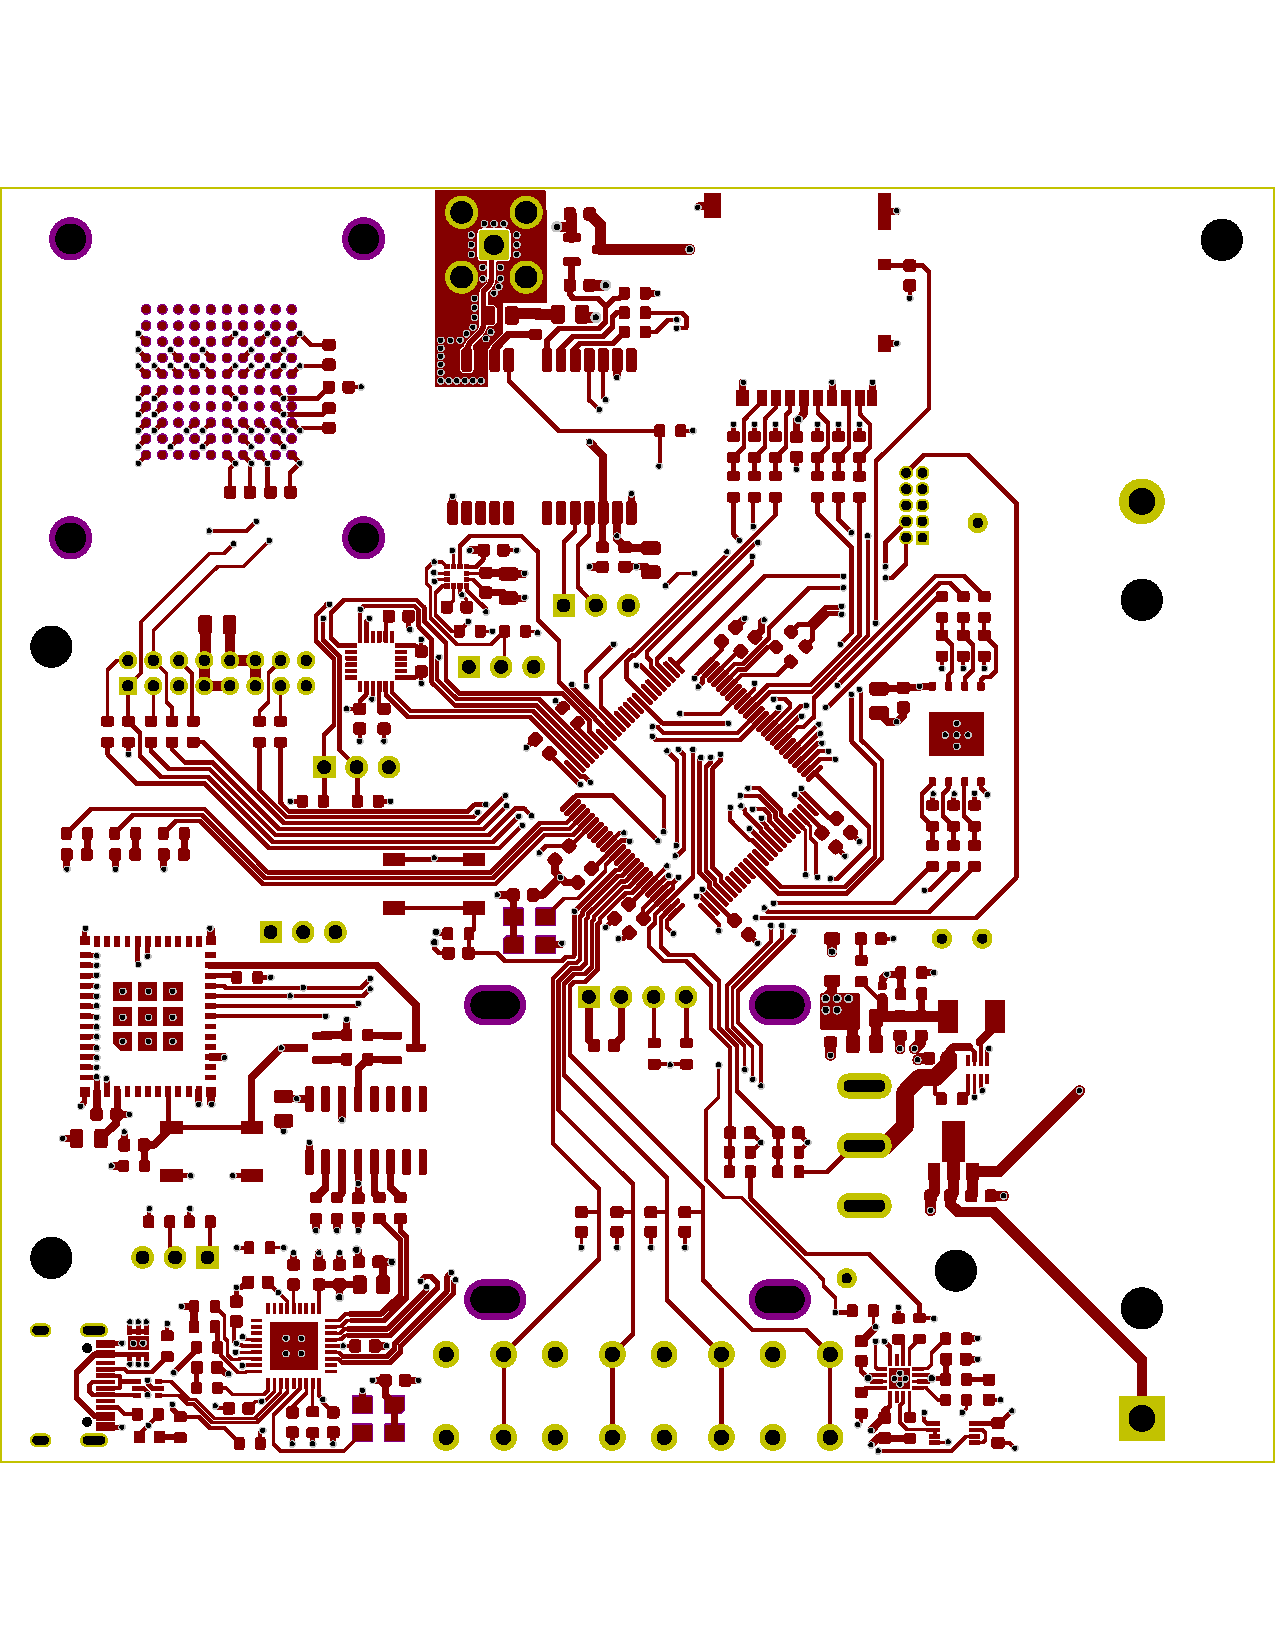
\includegraphics[width=\textwidth]{KiCad/boardF}

\section{Vnitřní vrstva mědi DPS In1}
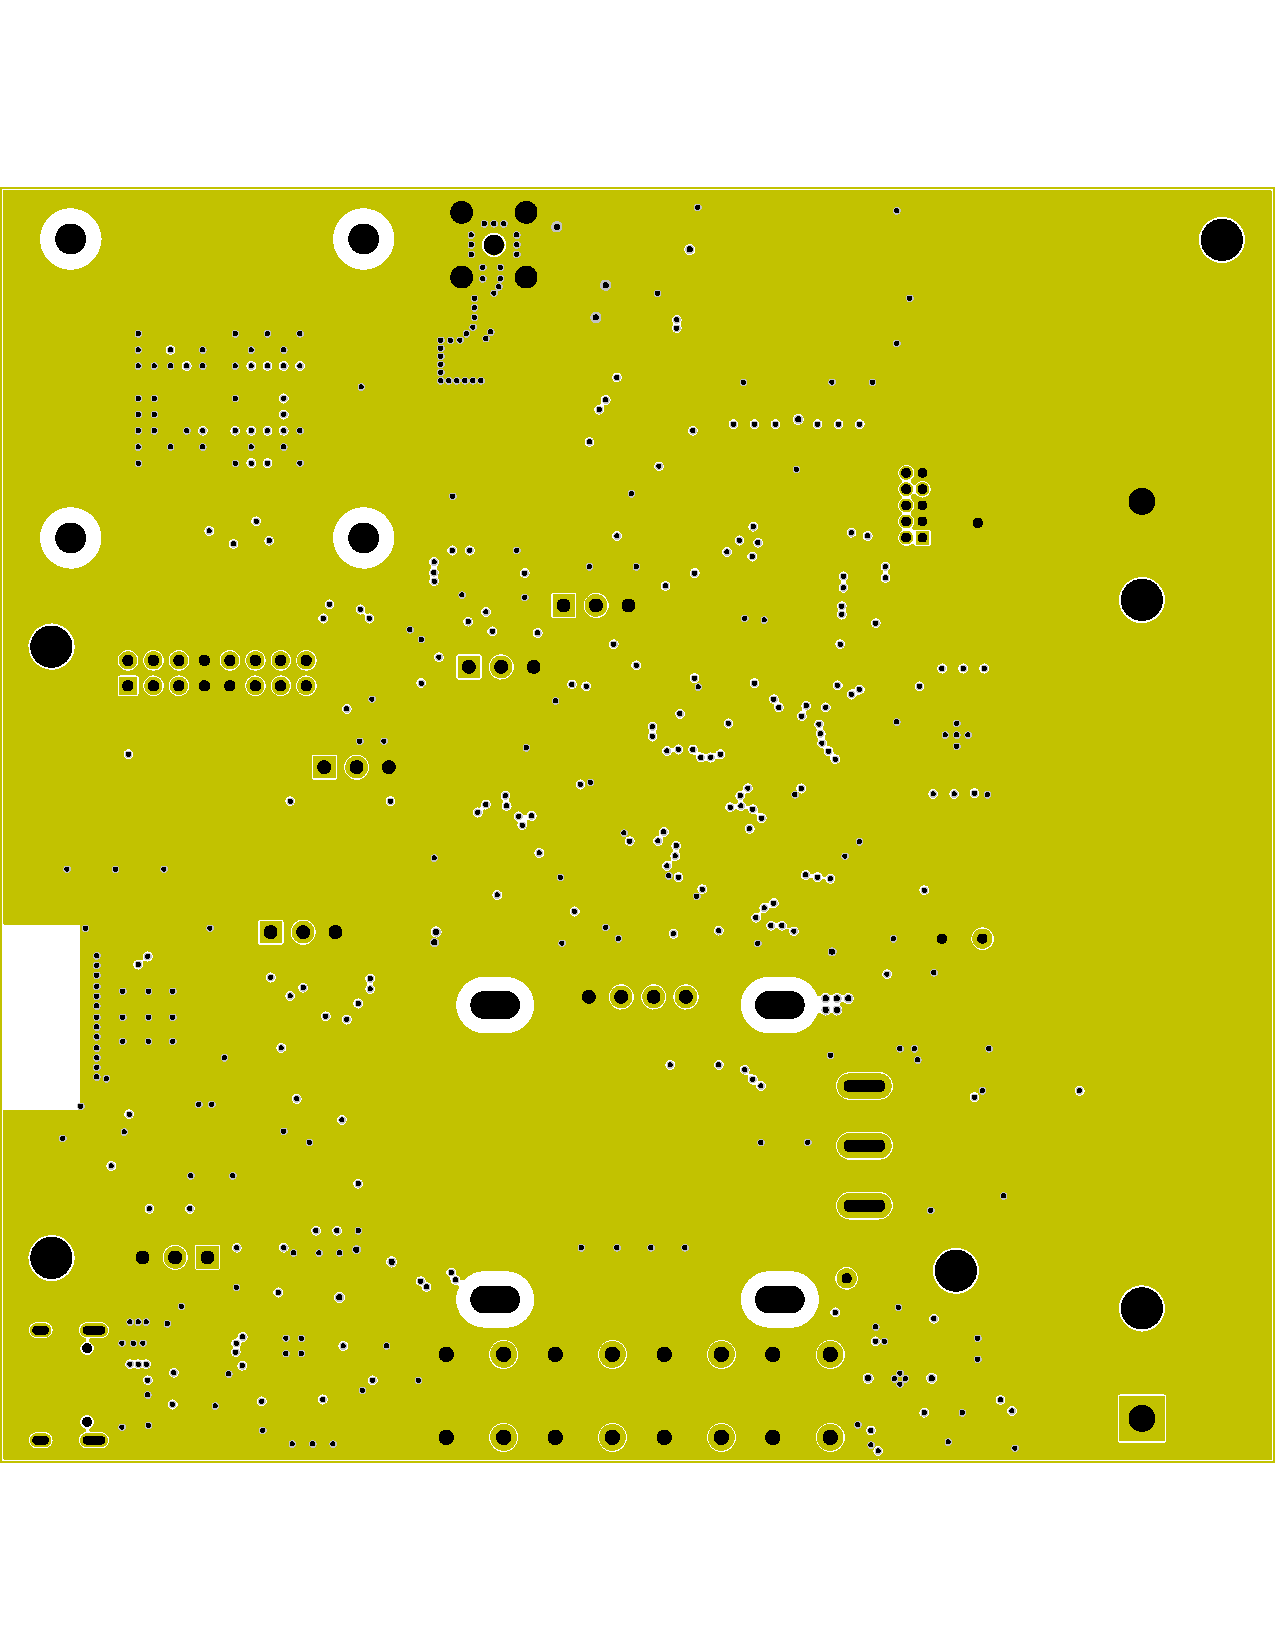
\includegraphics[width=\textwidth]{KiCad/boardIn1}

\section{Vnitřní vrstva mědi DPS In2}
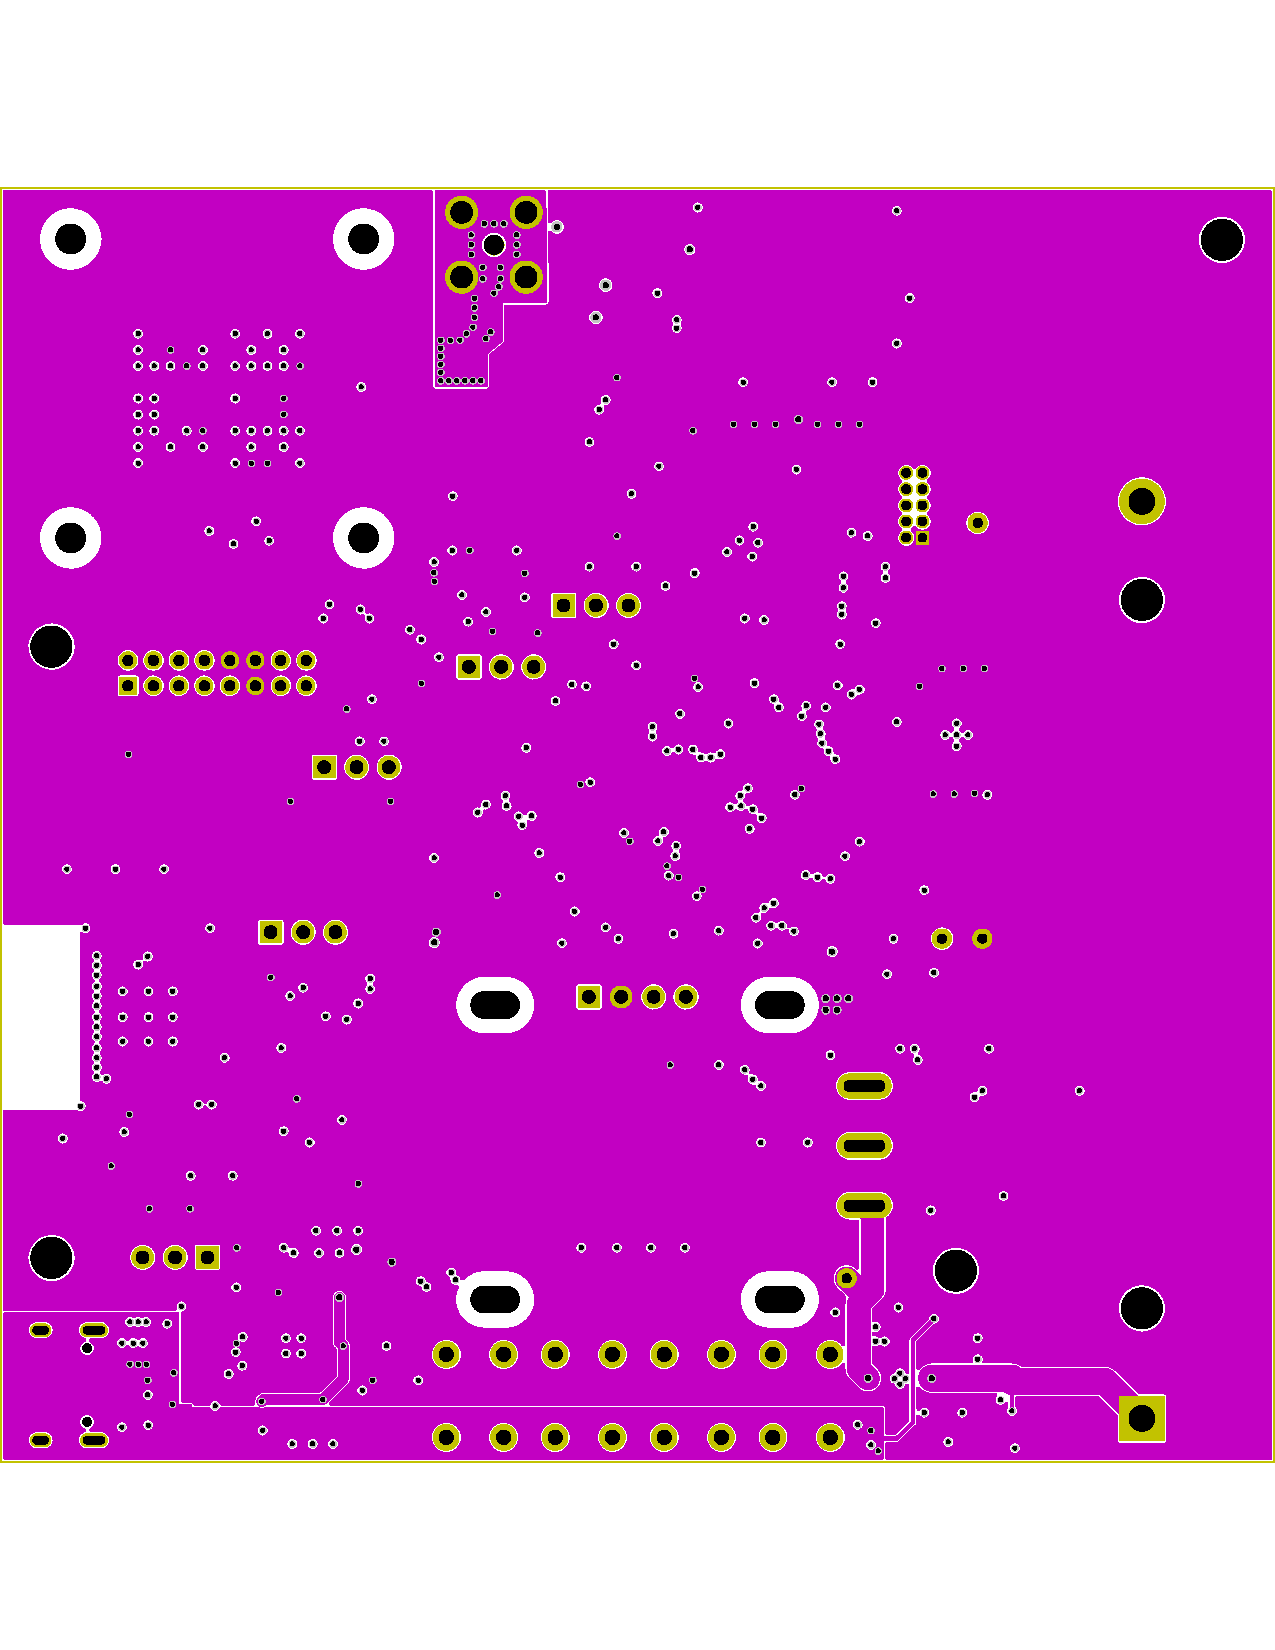
\includegraphics[width=\textwidth]{KiCad/boardIn2}

\section{Spodní vrstva mědi DPS} \label{BottomApp}
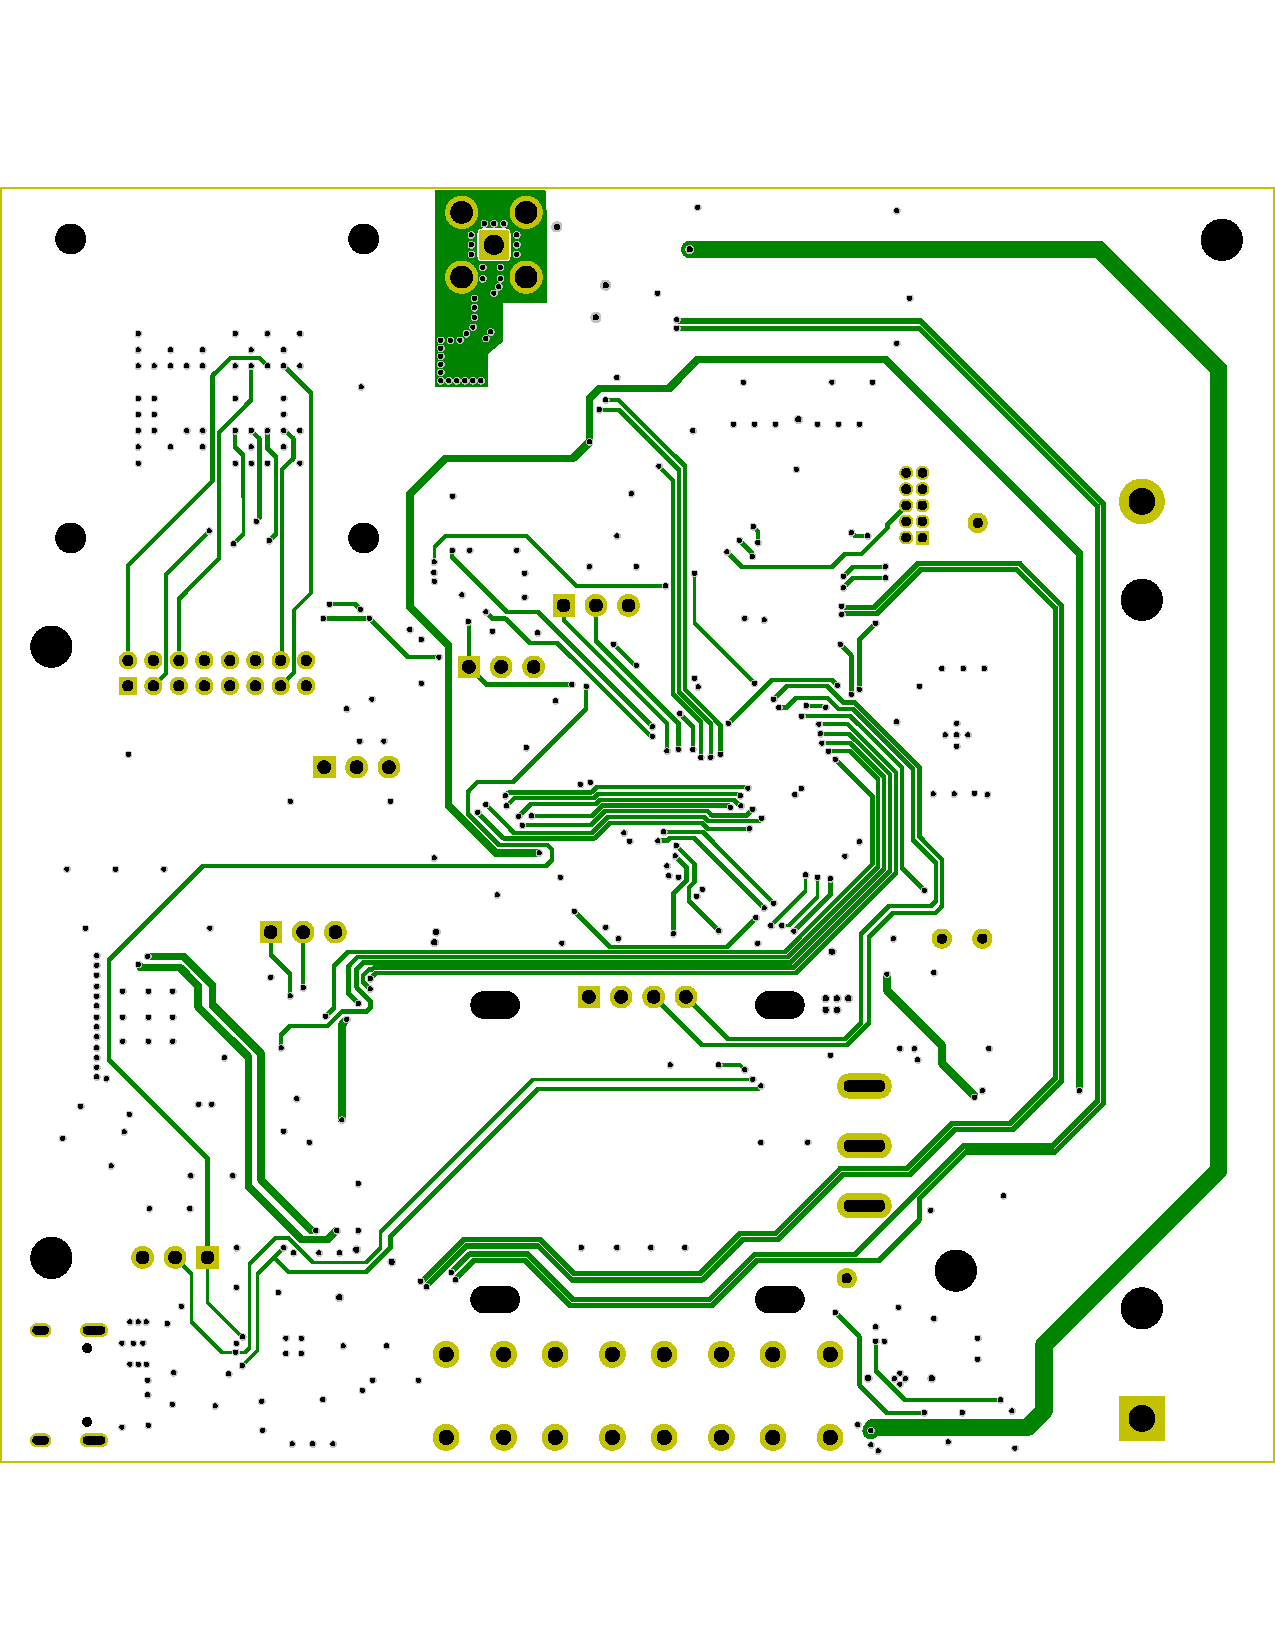
\includegraphics[width=\textwidth]{KiCad/boardB}




\end{document}